\section{Wellen}

\subsection{Definition}

Eine Welle ist eine \textbf{Störung eines Gleichgewichtszustandes}, die sich \textbf{im Raum ausbreitet}.


\subsubsection{Bemerkungen zur Definition}

\begin{itemize}
	\itemsep0em
	\item Voraussetzung für die \textbf{Ausbreitung} einer Welle ist die \\
		\textbf{Kopplung} benachbarter Teilchen.	
	\item \textbf{Eine Welle transportiert Energie (keine Materie)} 
	\item Die Störung kann von ganz unterschiedlicher Natur sein: 
		\begin{itemize}
			\item Druck in Luft
			\item Auslenkung einer Position entlang einem Seil (Saite)
			\item Elektrische Signale  
		\end{itemize}
\end{itemize}


\textbf{Die Störung wird mit $\xi$ beschrieben: $\xi = \xi(x, y, z, t)$}



\subsection{Klassifizierung von Wellen}

\begin{minipage}{0.45\linewidth}
Welle breitet sich \textbf{senkrecht} zur Störung aus \\

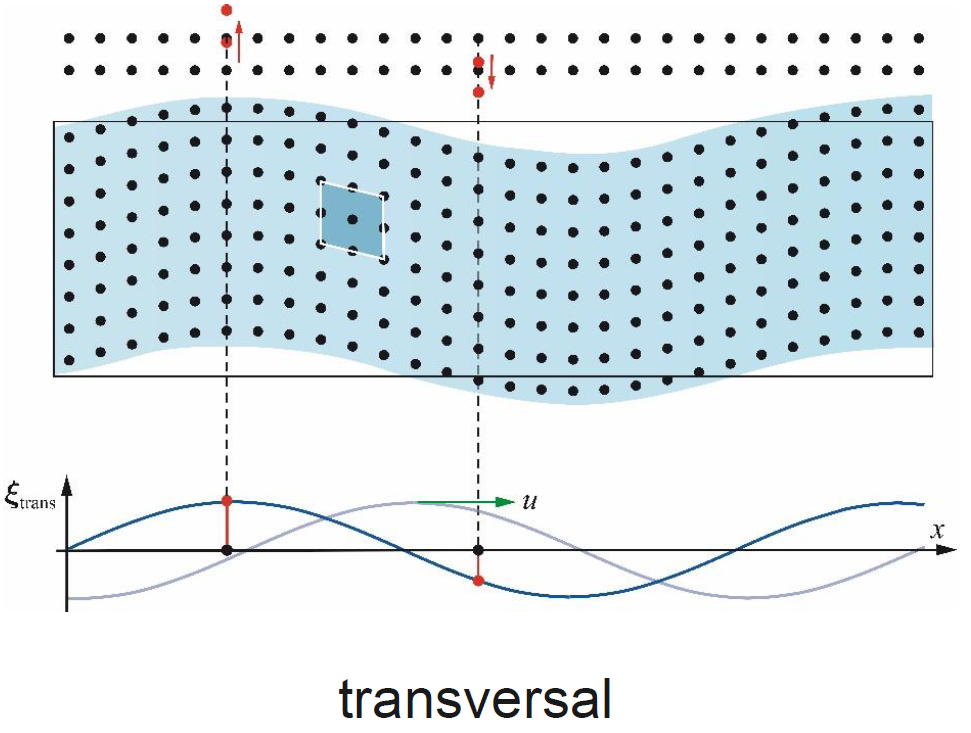
\includegraphics[width=0.95\linewidth]{Bilder/Wellen-Optik/welle_transversal} \\
z.B. Lichtwellen
\end{minipage}
\hfill
\begin{minipage}{0.45\linewidth}
Welle breitet sich \textbf{parallel} zur Störung aus \\

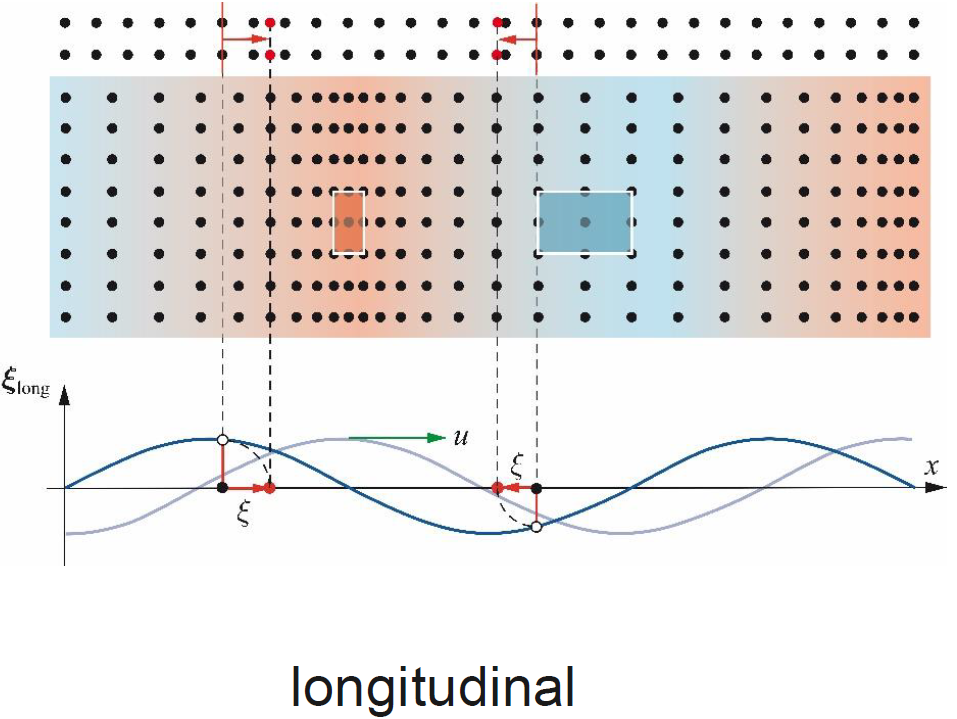
\includegraphics[width=0.95\linewidth]{Bilder/Wellen-Optik/welle_longitudinal}\\
z.B. Schallwellen

\end{minipage}

\subsection{Wellengeschwindigkeit / Phasengeschwindigkeit $u$}
Die Störung an der Position $x_0$ zum Zeitpunkt $t=0$ breitet sich mit der Geschwindigkeit $u$ aus und erreicht nach einer Zeit $t$ die Position $x$ \\

\center{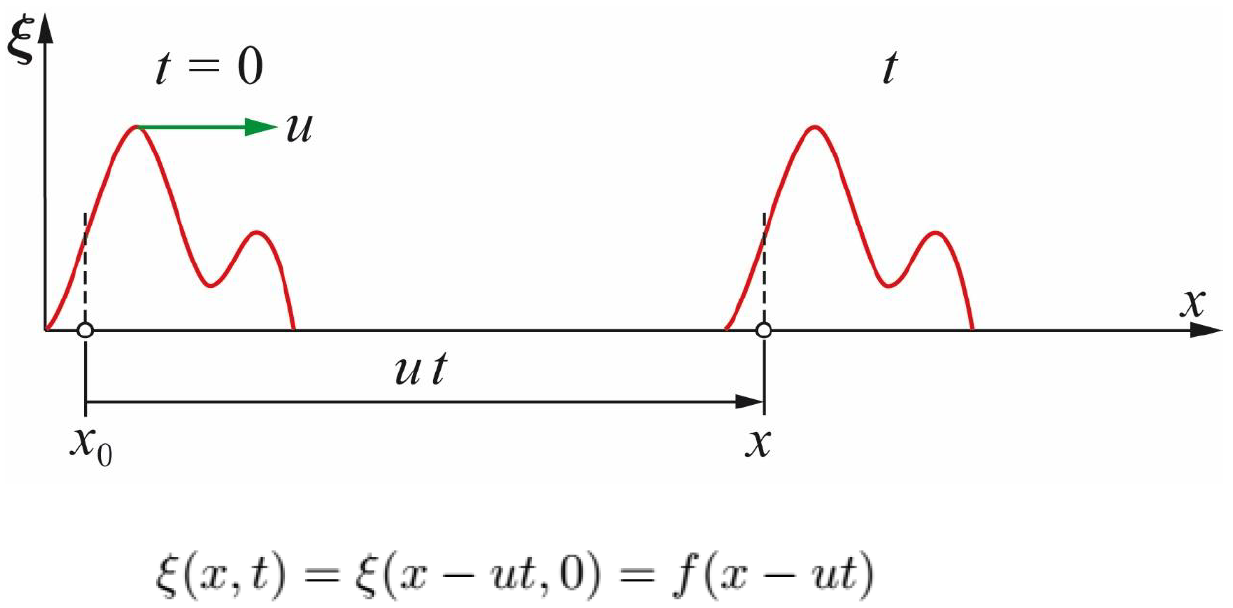
\includegraphics[width=0.7\linewidth]{Bilder/Wellen-Optik/ausbreitung_stoerung}} \\

\raggedright
\textbf{In einem Medium mit grösserer Dichte breiten sich Wellen schneller aus!} $\Rightarrow$ Bessere Kopplung der Moleküle \\
\vspace{0.5cm}

Man schaut bei der Beschreibung der Fortbewegung auf den Ort. Die Verschiebung des Ortes wird mit der Zeit hineingebracht

\subsubsection{Typische Wellengeschwindigkeiten}
\begin{tabular}{| l | c |}
	\hline
	\textbf{Material}   & \textbf{$m/s$} \\ \hline
	Wasser (20°C)       & 1300 \\ \hline
	Luft (20°C)         & 344 \\ \hline
	Kohlendioxid (20°C) & 258 \\ \hline
	Aluminium           & 5200 \\ \hline
	Eisen               & 5000 \\ \hline
	Tannenholz          & 3320 \\ \hline
	Beton               & 3100 \\ \hline
	Polystrol           & 1800 \\ \hline
	Kork                & 500 \\ \hline
	elektromagn. Welle  & 299'792'458 \\ \hline
\end{tabular}

% \vfill\null
% \columnbreak

\subsubsection{Verschiedene Wellengeschwindigkeiten}

\begin{minipage}{0.45\linewidth}
Schallwellen in Fluiden: 
\end{minipage}
\hfill
\begin{minipage}{0.48\linewidth}
$$\boxed{ u = \sqrt{\frac{1}{\rho \, \kappa}} }$$
\end{minipage}


\begin{minipage}{0.45\linewidth}
Schallwellen in Gasen:
\end{minipage}
\hfill
\begin{minipage}{0.48\linewidth}
$$\boxed{ u = \sqrt{\frac{\varkappa \, p}{\rho}} = \sqrt{\frac{\varkappa \, R \, T}{M}} }$$
\end{minipage}


\begin{minipage}{0.45\linewidth}
Elastische Longitudinalwellen in einem schlanken Stab
\end{minipage}
\hfill
\begin{minipage}{0.48\linewidth}
$$\boxed{ u = \sqrt{\frac{E}{\rho}} }$$
\end{minipage}

\begin{minipage}{0.45\linewidth}
Elastische Transversalwellen
\end{minipage}
\hfill
\begin{minipage}{0.48\linewidth}
$$\boxed{ u = \sqrt{\frac{G}{\rho}} }$$
\end{minipage}

\begin{minipage}{0.45\linewidth}
Transversalwellen auf einem Seil oder einer Saite
\end{minipage}
\hfill
\begin{minipage}{0.48\linewidth}
$$\boxed{ u = \sqrt{\frac{F}{\rho \, A}} }$$ 
\end{minipage}

\begin{minipage}{0.45\linewidth}
Elektromagnetische Wellen (transversal) \\
(z.B. Lichtwellen)
\end{minipage}
\hfill
\begin{minipage}{0.48\linewidth}
$$\boxed{ u = \frac{c}{n} }$$ \\
\end{minipage}


\renewcommand{\arraystretch}{1.1}
\begin{tabular}{c l c}
$u$ & Wellengeschwindigkeit & $[u] = \frac{\m}{\s}$ \\
$A$ & Querschnittsfläche & $[A] = \m^2$ \\
$E$ & Elastizitätsmodul & $[E] = \frac{\N}{\m^2} = \Pa$\\
$F$ & Spannkraft des Seils / der Saite & $[F] = \N$ \\
$G$ & Schubmodul & $[G] = \frac{\N}{\m^2} = \Pa$ \\
$M$ & Molmasse & $[M] = \frac{\kg}{\mol}$ \\
$p$ & Druck & $[p] = \Pa$ \\
$R$ & Universelle Gaskonstante: $R = 8.314 \mathrm{\frac{J}{mol \cdot K}}$ & $[R] = \mathrm{\frac{J}{mol \cdot K}} $ \\
$T$ & \textbf{Absolut-}Temperatur (in K) & $[T] = \mathrm{K}$ \\
$\kappa$ & Kompressibilität & $[\kappa] = \frac{1}{\Pa}$ \\
$\varkappa$ & Adiabatenexponent & $[\varkappa] = 1$ \\
$\rho$ & Dichte & $[\rho] = \frac{\kg}{\m^3}$ \\
$n$ & Brechungsindex & $[n] = 1$ \\
$c$ & Lichtgeschwindigkeit: $c = 300 \cdot 10^6 \, \frac{\m}{\s}$ & $[c] = \frac{\m}{\s}$ \\
\end{tabular}
\renewcommand{\arraystretch}{1}



\subsection{Wellengleichungen}
Die Wellengleichungen stellen eine \textbf{Verbindung zwischen Zeit und Ort} her \\

\vspace{0.5cm}


\begin{minipage}{0.45\linewidth}
Eindimensional \\
Welle breitet sich in 1D aus \\
\end{minipage}
\hfill
\begin{minipage}{0.48\linewidth}
$$\boxed{ \frac{\partial^2 \xi}{\partial x^2} = \frac{1}{u^2} \frac{\partial^2 \xi}{\partial t^2}  }$$  \\
\end{minipage}


\begin{minipage}{0.45\linewidth}
Zweidimensional \\
Welle breitet sich in 2D aus \\
\end{minipage}
\hfill
\begin{minipage}{0.48\linewidth}
$$\boxed{ \frac{\partial^2 \xi}{\partial x^2} + \frac{\partial^2 \xi}{\partial y^2} = \frac{1}{u^2} \frac{\partial^2 \xi}{\partial t^2}  }$$  \\
\end{minipage}


% \vfill\null
% \columnbreak


\begin{minipage}{0.45\linewidth}
Dreidimensional \\
Welle breitet sich in 3D aus \\
\end{minipage}
\hfill
\begin{minipage}{0.48\linewidth}
$$\boxed{ \frac{\partial^2 \xi}{\partial x^2} + \frac{\partial^2 \xi}{\partial y^2} + \frac{\partial^2 \xi}{\partial z^2} = \frac{1}{u^2} \frac{\partial^2 \xi}{\partial t^2}  }$$ \\
\end{minipage}



\subsubsection{Wichtige Lösung der Wellengleichung (1D)}

\begin{minipage}{0.38\linewidth}
$$\frac{\partial^2 \xi}{\partial x^2} = \frac{1}{u^2} \frac{\partial^2 \xi}{\partial t^2} $$ \\
\end{minipage}
\hfill
\begin{minipage}{0.58\linewidth}
Ansatz: $\xi(x,t) = \xi_0 \cdot \sin(\omega \, t - k \, x)$ \\
\end{minipage}

$$ \underbrace{- k^2 \, A \, \sin(\omega \, t - k \, x)}_{\substack{\frac{\partial^2 \xi}{\partial x^2} }} = - \frac{1}{u^2} \cdot \underbrace{ \omega^2 \, A \,\sin(\omega \, t - k \, x)}_{\substack{\frac{\partial^2 \xi}{\partial t^2} }}  $$ 


$$ \boxed{ \text{mit Lösung } u^2 = \frac{\omega^2}{k^2} } $$



\subsection{Harmonische Wellen}

$$ \boxed{ \xi(x, t) = \xi_0 \cdot \sin( \omega \, t - k \, x + \varphi) }  $$


\subsubsection{Terminologie}

\center{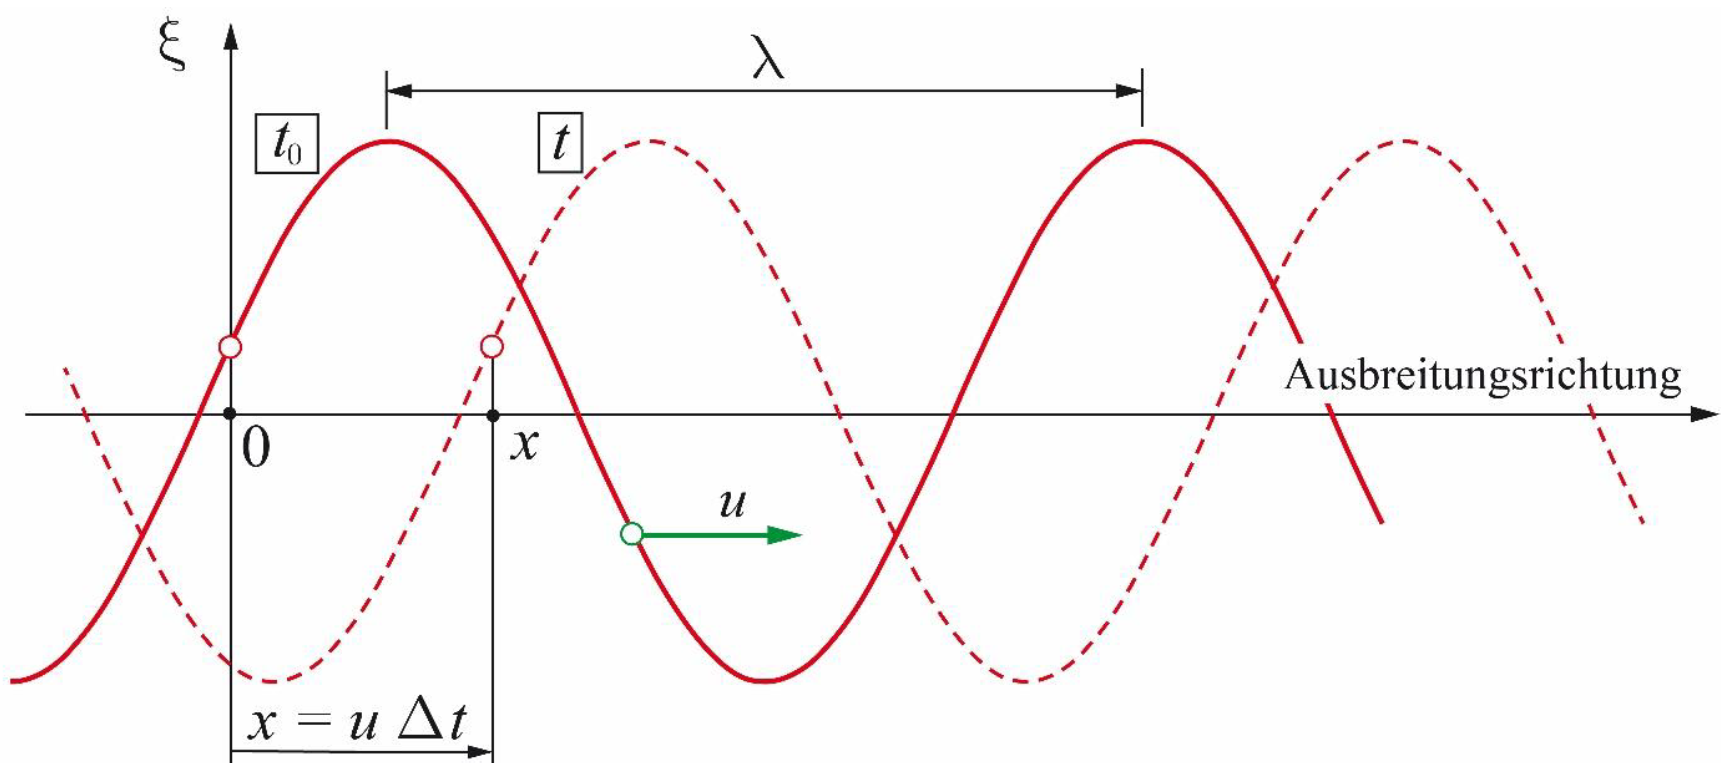
\includegraphics[width=0.7\linewidth]{Bilder/Wellen-Optik/harmonische_wellen_terminologie}} \\
\raggedright

\renewcommand{\arraystretch}{1.1}
\begin{tabular}{c l c}
$\xi_0$ & Amplitude & $[\xi_0]$ \\
$\omega$ & Kreisfrequentz & $[\omega] = \frac{\rad}{\s}$ \\
$T$ & Periodendauer & $[T] = \s$ \\
$k$ & Wellenzahl & $[k] = \frac{1}{\m}$ \\
$\lambda$ & Wellenlänge & $\lambda = \m $ \\
$u$ & Wellengeschwindigkeit & $[u] = \frac{\m}{\s}$ \\
$\varphi$ & Phasenverschiebung & $[\varphi] = \rad$ 
\end{tabular}
\renewcommand{\arraystretch}{1}



\subsubsection{Zusammenhänge}
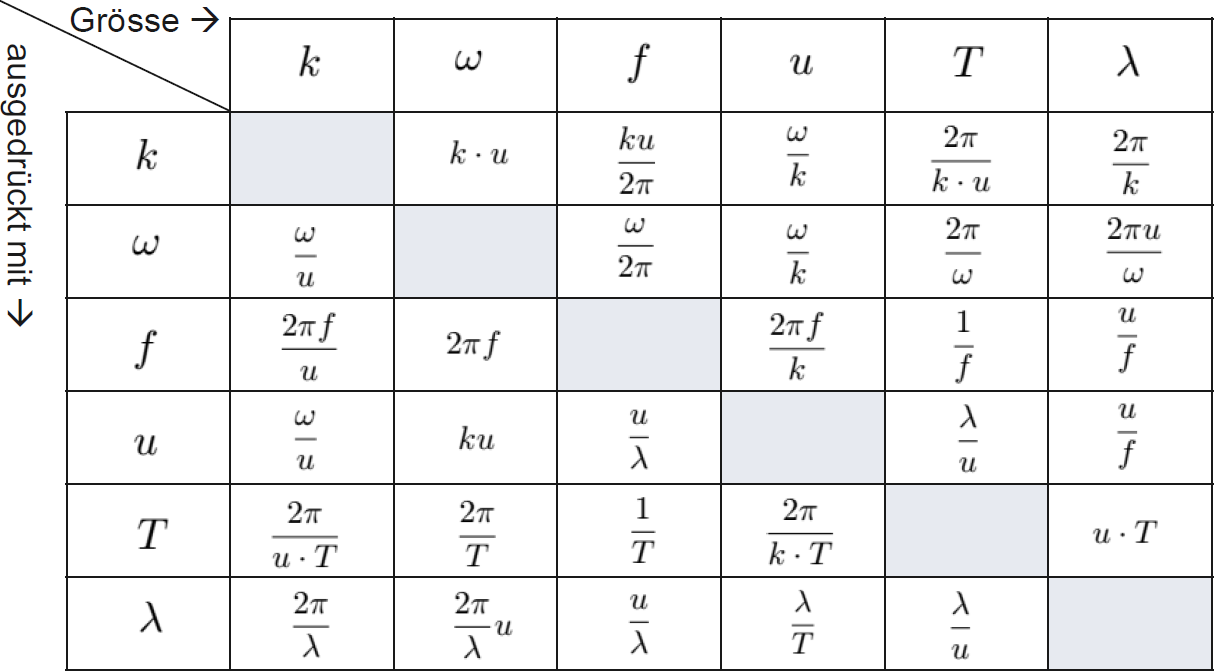
\includegraphics[width=0.8\linewidth]{Bilder/Wellen-Optik/harmonische_wellen_zusammenhaenge}






\subsection{Wellenflächen / Wellenfronten}
Die Gesamtheit aller Punkte, die zu einer bestimmten Zeit im gleichen Schwingungszustand sind, bilden eine Fläche im Raum. \\

Diese \textbf{Flächen mit gleicher Phase} werden als \textbf{Wellenflächen} oder \textbf{Wellenfronten} genannt.\\
\vspace{0.2cm}

Eine Welle kann sich in 3 Dimensionen ausbreiten und dabei \textbf{verschiedene Wellenflächen} zeigen. 




\subsection{Wellenausbreitung}

\begin{minipage}{0.25\linewidth}
Wellengleichung (3D)
\end{minipage}
\hfill
\begin{minipage}{0.73\linewidth}
$$\boxed{ \frac{\partial^2 \xi}{\partial x^2} + \frac{\partial^2 \xi}{\partial y^2} + \frac{\partial^2 \xi}{\partial z^2} = \frac{1}{u^2} \frac{\partial^2 \xi}{\partial t^2}  }$$
\end{minipage}

\begin{minipage}{0.25\linewidth}
Lösungsansatz \\
\end{minipage}
\hfill
\begin{minipage}{0.73\linewidth}
$$ \boxed{ \xi = \xi_0 \e^{\jimg \, (\omega \, t - \vec{k} \bullet \vec{r})} }$$ \\
\end{minipage}

mit Wellenvektor $\vec{k} = \begin{pmatrix} k_x \\ k_y \\ k_z  \end{pmatrix}$ und Ortsvektor $ \vec{r} = \begin{pmatrix} r_x \\ r_y \\ r_z  \end{pmatrix}$




\subsubsection{Ebene Wellen}

\begin{minipage}{0.3\linewidth}
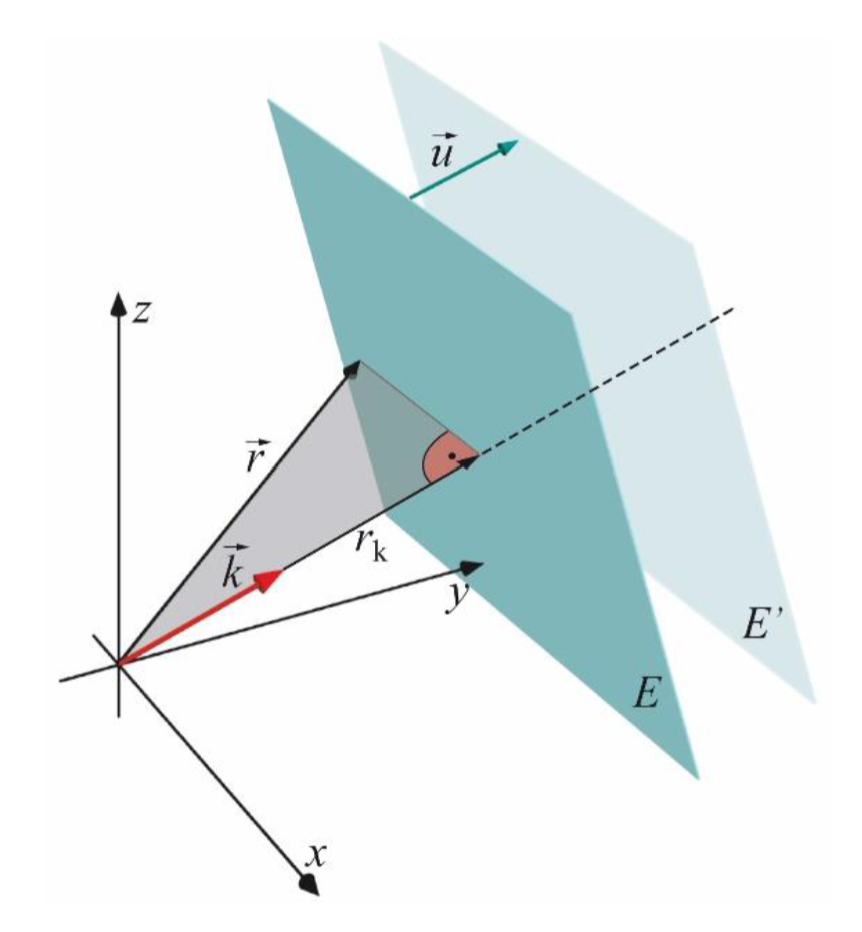
\includegraphics[width=0.98\linewidth]{Bilder/Wellen-Optik/Ebene_Welle}
\end{minipage}
\hfill
\begin{minipage}{0.68\linewidth}

\begin{itemize}
	\item Wellenfronten sind Ebenen im Raum 
	\item Wellenvektor $\vec{k}$ steht senkrecht auf \\
		der Ebenen 
	\item \textbf{Abstand} zw. zwei Wellenfronten ist $\lambda$ 

\end{itemize}


Die Ebenen bewegen sich mit der \\
Wellengeschwindigkeit
$$ \boxed{ u = \frac{\omega}{k} \text{ mit } k = ||\vec{k}|| = \sqrt{k_x^2 + k_y^2 + k_z^2} }$$  in die \textbf{Richtung}, die durch den \textbf{Wellenvektor} $\vec{k}$ gegeben ist.
\end{minipage}




\subsubsection{Kugelwellen}

\begin{minipage}{0.3\linewidth}
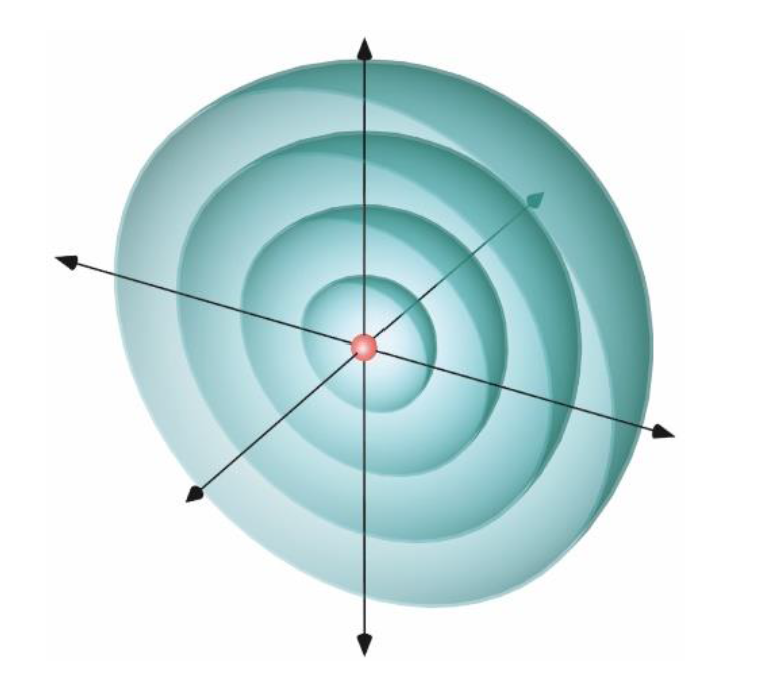
\includegraphics[width=0.98\linewidth]{Bilder/Wellen-Optik/Kugel_Welle}
\end{minipage}
\hfill
\begin{minipage}{0.68\linewidth}

\begin{itemize}
	\item Wellenfronten sind Kugeln 
	\item Wellenvektor $\vec{k}$ steht senkrecht auf  \\
 		Wellenfronten 
	\item Wellenfronten bewegen sich mit der \\
		 Wellengeschwindigkeit vom Zentrum weg 
	\item Amplitude nimmt mit $\frac{1}{r}$ ab \\
\end{itemize}
\end{minipage}

Für eine \textbf{punktförmige Quelle} und \textbf{keine Winkelabhängigkeit} gilt:

$$ \boxed{ \frac{1}{u^2} \frac{\partial^2 \xi}{\partial t^2} = \frac{2}{r} \Big( \frac{\partial \xi}{\partial r} \Big) + \frac{\partial^2 \xi}{\partial r^2} }$$

$$ \boxed{  \text{mit Lösungsansatz } \xi(t, r) = \frac{1}{r} \xi_0 \, \e^{\jimg \, (\omega \, t - k \, r)} }  $$

% \vfill\null
% \columnbreak




\subsection{Bewegte Quellen}

	\begin{minipage}{0.48\linewidth}
		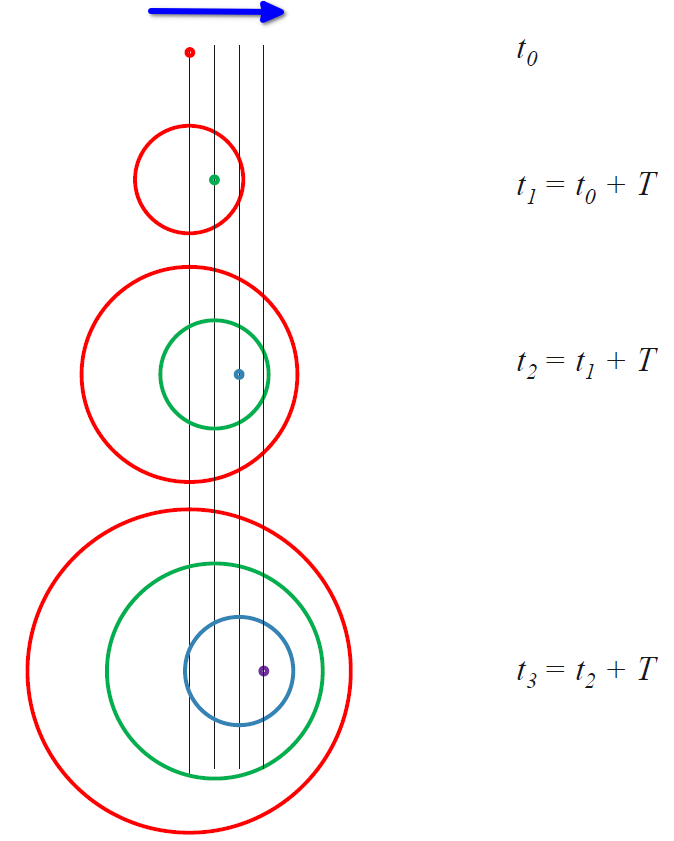
\includegraphics[width=0.98\linewidth]{Bilder/Wellen-Optik/Bewegte_Quellen}
	\end{minipage}
	\hfill
	\begin{minipage}{0.48\linewidth}
		Die Quelle bewegt sich mit der \textcolor{blue}{Geschwindigkeit $v_Q$} in \\ eingezeichneter Richtung fort\\

		Die Quelle verschiebt sich in der Zeit $T$ um 
		$$ \boxed{ \Delta x = v_Q \cdot T }$$
	\end{minipage}

\subsubsection{Doppler Effekt}
	Die \textbf{Veränderung der Wellenlänge} $\lambda$ der von einer \textbf{bewegten Quelle} ausgesandten Wellen ist als \textbf{Doppler Effekt} bekannt.  \\

	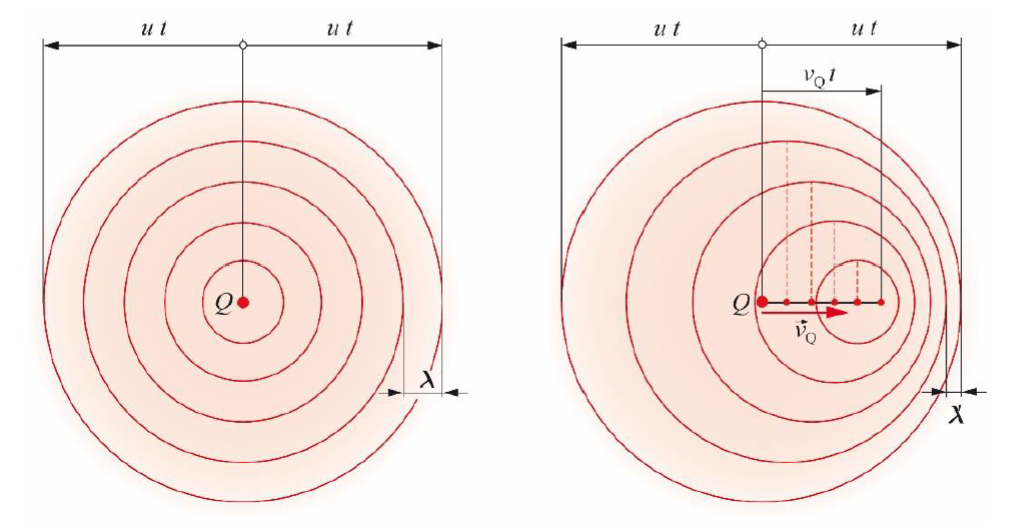
\includegraphics[width=0.8\linewidth]{Bilder/Wellen-Optik/Doppler_effekt}

\subsubsection{Bewegte Quelle vs. unbewegte Quelle}

	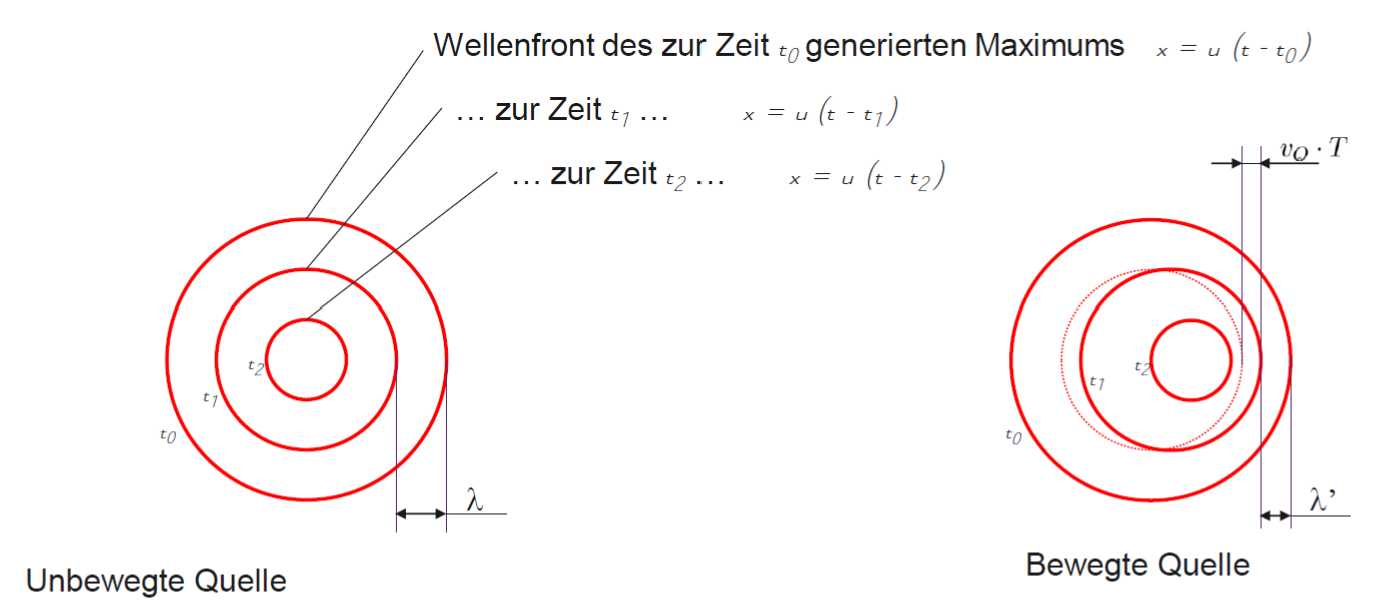
\includegraphics[width=0.98\linewidth]{Bilder/Wellen-Optik/Unbewegte_Quelle}

\subsection{Frequenzverschiebung durch Bewegung}

	Die Quelle sendet eine Frequenz $f$ aus. Durch die Bewegung der Quelle ändert sich die Wellenlänge $\lambda$ und somit ergibt sich eine neue Frequenz $f'$, welche ein statischer Beobachter wahrnimmt. 

	Falls $v$ nicht parallel zur Beobachtungsrichtung ist, siehe \textbf{\ref{bewegte-Quelle-mit-Winkel}}

\begin{align*}
\lambda' &= \lambda -v_{Q_{||}} \cdot T  \\
\lambda'&= \lambda -v_{Q_{||}} \frac{\lambda}{u}\\
\lambda' &= \lambda \left(1 - \frac{v_{Q_{||}}}{u}\right)  \\
f'&= \frac{u}{\lambda'} = \frac{u}{\lambda\left(1-\frac{v_{Q_{||}}}{u}\right)} = \frac{f}{\left(1-\frac{v_{Q_{||}}}{u}\right)}
\end{align*}

\subsection{Bewegte Quelle oder bewegter Beobachter}

\begin{minipage}{0.48\linewidth}
	\begin{center}
		Bewegte Quelle:
		$$ \boxed{f' = \frac{1}{\left(1 \mp \frac{v_{Q_{||}}}{u}\right)}f}$$
	\end{center}
\end{minipage}
\hfill
\begin{minipage}{0.48\linewidth}
	\begin{center}
		Bewegter Beobachter:
		$$ \boxed{f' = \left( 1 \pm \frac{v_{B_{||}}}{u}  \right) \, f }$$\\
	\end{center}
\end{minipage}


\begin{tabular}{ll}
+ & Quelle bewegt sich weg / Beobachter bewegt sich hin\\
- & Quelle bewegt sich hin / Beobachter bewegt sich weg\\
\\
\end{tabular}


\begin{tabular}{clc}
$\lambda$ & Wellenlänge der aussendeten Welle & $[\lambda] = \m$ \\
$\lambda'$ & Wellenlänge der wahrgenommenen Welle & $[\lambda'] = \m$ \\
$v_{Q_{||}}$ & Geschwindigkeit der bewegten Quelle & $[v_{Q_{||}}] = \frac{\m}{\s}$ \\
$v_{B_{||}}$ & Geschwindigkeit des bewegten Beobachters & $[v_{Q_{||}}] = \frac{\m}{\s}$ \\
$u$ & Wellengeschwindigkeit & $[u] = \frac{\m}{\s}$ \\
$f$ & Frequenz der ausgesendeten Wellen & $[f] = \Hz$ \\
$f'$ & Frequenz der wahrgenommenen Wellen & $[f'] = \Hz$ \\
$T$ & Periodendauer (Dauer der Ausbreitung) & $[T] = \s$ \\
\end{tabular}






\subsection{Bewegte Quelle mit Winkel}\label{bewegte-Quelle-mit-Winkel}
Die Quelle bewegt sich nicht direkt auf den Beobachter zu, sondern sie bewegt sich am \textbf{Beobachter vorbei} \\


\begin{minipage}{0.48\linewidth}
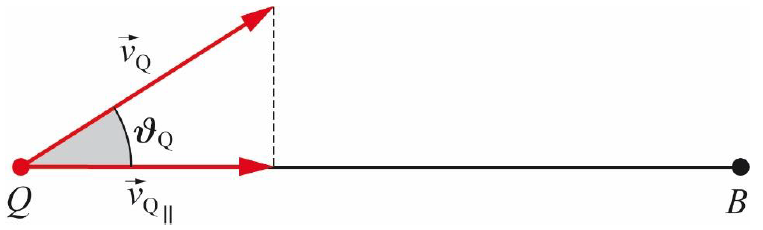
\includegraphics[width=0.98\linewidth]{Bilder/Wellen-Optik/bewegte_quelle_winkel} \\
\end{minipage}
\hfill
\begin{minipage}{0.48\linewidth}
$$ \boxed{ f' =  \frac{1}{1 - \frac{v_Q}{u} \cdot \cos(v_Q)}  \, f} $$
\end{minipage}



\begin{tabular}{clc}
$v_Q$ & Geschwindigkeit der bewegten Quelle & $[v_Q] = \frac{\m}{\s}$ \\
$u$ & Wellengeschwindigkeit & $[u] = \frac{\m}{\s}$ \\
$f$ & Frequenz der ausgesendeten Wellen & $[f] = \Hz$ \\
$f'$ & Frequenz der wahrgenommenen Wellen & $[f'] = \Hz$ \\
\end{tabular}

% \vfill\null
% \columnbreak


\subsubsection{Beispiel Winkel zw. Quelle und Beobachter}

\begin{minipage}{0.48\linewidth}
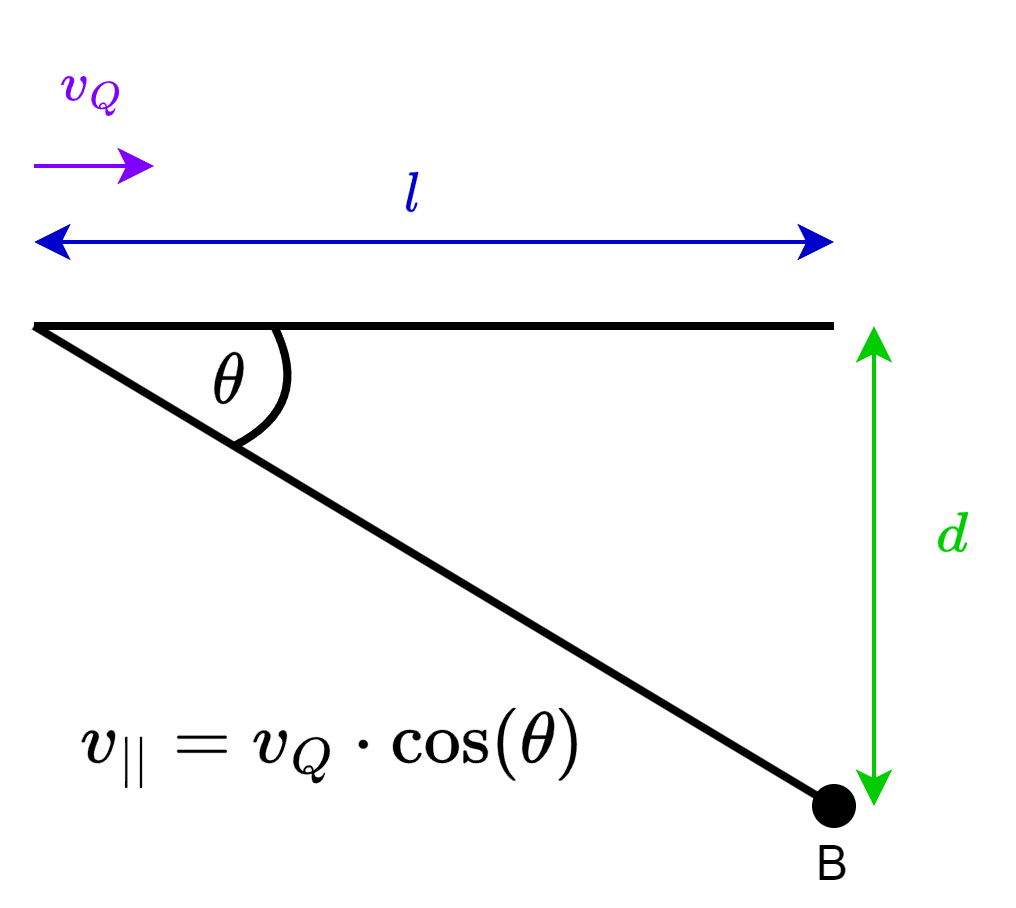
\includegraphics[width=0.98\linewidth]{Bilder/Wellen-Optik/beispiel_bewegte_quelle} \\
\vspace{2.5cm}
\end{minipage}
\hfill
\begin{minipage}{0.48\linewidth}
\textbf{Gegeben:} $v_Q, \, \theta, \,u, \,d, \,l$ \\
\textbf{Gesucht:} $\frac{f'}{f}$ \\

$f' =  \frac{1}{1 - \frac{v_Q}{u} \cdot \cos(v_Q)}$ \\
$\tan(\theta) = \frac{d}{l} =  \frac{\sin(\theta)}{\cos(\theta)}$ \\
$\sin^2(\theta) = 1 - \cos^2(\theta)$ \\
\vspace{0.2cm}


$\Rightarrow \tan(\theta) = \frac{d}{l} = \frac{\sqrt{ 1 - \cos^2(\theta)}}{\cos(\theta)} $ \\

$ \frac{1}{\cos^2(\theta)} = \frac{d^2}{l^2} + 1 $ \\

$\cos^2(\theta) = \frac{1}{1 + \frac{d^2}{l^2}}$ \\

$\boxed{ \Rightarrow \frac{f'}{f} = \frac{1}{1 - \frac{v_Q}{u} \cdot \sqrt{\frac{l^2}{l^2 + d^2} } } } $

\end{minipage}




\subsection{Bewegte Quelle und bewegter Beobachter}

\begin{minipage}{0.48\linewidth}
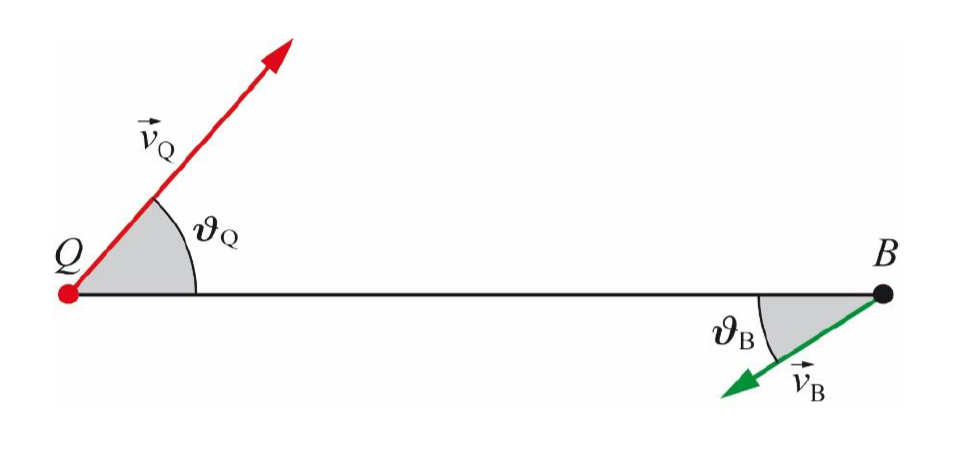
\includegraphics[width=0.98\linewidth]{Bilder/Wellen-Optik/akustischer_doppler_effekt} \\
\end{minipage}
\hfill
\begin{minipage}{0.48\linewidth}
$$ \boxed{f_B = \frac{u+ v_B \cos(\vartheta_B)}{u- v_Q \cos(\vartheta_Q)}f_Q} $$
\end{minipage}

\renewcommand{\arraystretch}{1.1}
\begin{tabular}{clc}
$\vartheta_B = \theta_B$ & siehe Skizze & $[\vartheta_B] = $°\\
$v_B$ & Geschwindigkeit bewegter Beobachter & $[v_B] = \frac{\m}{\s}$ \\
$\vartheta_Q = \theta_Q$ & siehe Skizze & $[\vartheta_Q] = $°\\
$v_Q$ & Geschwindigkeit bewegte Quelle & $[v_Q] = \frac{\m}{\s}$ \\
$u$ & Wellengeschwindigkeit & $[u] = \frac{\m}{\s}$ \\
$f_B$ & Frequenz beim bewegten Beobachter & $[f_B] = \Hz$ \\
$f_Q$ & Frequenz bei der bewegten Quelle & $[f_Q] = \Hz$ \\
\end{tabular}
\renewcommand{\arraystretch}{1}

% \vfill\null
% \columnbreak


\subsubsection{Optischer Doppler Effekt}

\textbf{Wird verwendet, wenn die Wellengeschwindigkeit $\boldsymbol{u}$ gleich der Lichtgeschwindigkeit $\boldsymbol{c}$ ist!} \\

Es spielt nur die \textbf{relative} Bewegung von Beobachter und Quellen eine Rolle

$$ \boxed{f' = \frac{\sqrt{1-\beta^2}}{1 - \beta \cos(\vartheta)}f \text{ mit } \beta = \frac{v}{c} } $$


$$ \text{für } \beta << 1 \quad f' \simeq \frac{1}{1- \beta \cdot \cos(\theta)} \cdot f  $$

$$ \text{für } \beta << 1 \text{ und } \theta \approx \frac{\pi}{2} \quad f' \simeq \frac{1}{1- \beta } \cdot f $$



\subsubsection{Mach'scher Kegel}
Wenn sich die Quelle schneller fortbewegt als die Wellengeschwindigkeit, dann entsteht ein Mach'scher Kegel \\



\begin{minipage}{0.6\linewidth}
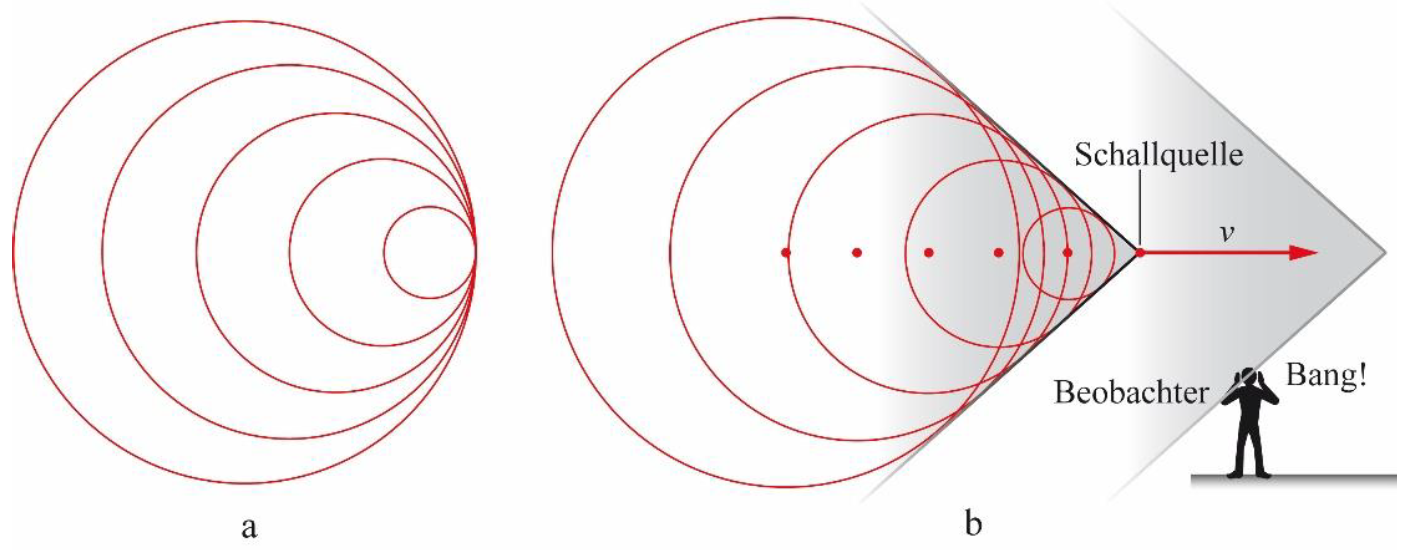
\includegraphics[width=0.95\linewidth]{Bilder/Wellen-Optik/machkegel_1} \\
\end{minipage}
\hfill
\begin{minipage}{0.38\linewidth}
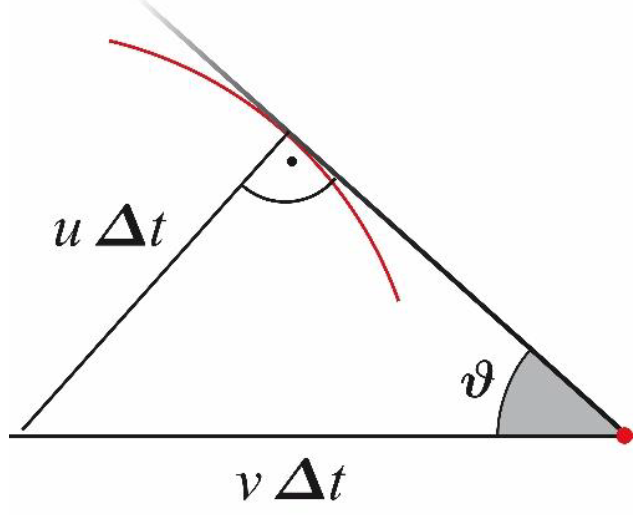
\includegraphics[width=0.95\linewidth]{Bilder/Wellen-Optik/machkegel_2} \\
\end{minipage}


\begin{minipage}{0.48\linewidth}
$$ \boxed{ \sin(\vartheta) = \frac{u \, \Delta t}{v \, \Delta t} = \frac{u}{v} } $$ \\
\end{minipage}
\hfill
\begin{minipage}{0.48\linewidth}
$$ \boxed{ M = \frac{v}{u} } $$ \\
\end{minipage}


\renewcommand{\arraystretch}{1.1}
\begin{tabular}{clc}
$v$ & Geschwindigkeit der Quelle & $[v] = \frac{\m}{\s}$ \\
$u$ & Wellengeschwindigkeit (Schallgeschwindingkeit) & $[u] = \frac{\m}{\s}$ \\
$M$ & Machzahl & $[M] = 1$
\end{tabular}
\renewcommand{\arraystretch}{1}



\subsection{Wellenwiderstand, Energietransport -- Schallwellen}

\subsubsection{Terminologie Wellenwiderstand}
Der \textbf{Wellenwiderstand $Z$} (auch \textbf{Impedanz} genannt) beschreibt, wie ein Medium den Fluss
von Energie beeinflusst. \\
\vspace{0.3cm}
$\Rightarrow$ 'Wie gut können sich Wellen in einem Medium ausbreiten?'

$$ \boxed{ Z = \rho \cdot u = \frac{\Delta p_0}{v_0} } $$

\vspace{0.2cm}

\renewcommand{\arraystretch}{1.2}
\begin{tabular}{clc}
$Z$ & Wellenwiderstand bzw. Impedanz & $[Z] = \Ohm = \frac{\Pa}{\m / \s} = \frac{\N \, \s}{\m^3}$ \\
$\rho$ & Dichte des Mediums & $[\rho] = \frac{\kg}{\m^3}$ \\
$u$ & Wellengeschwindigkeit & $[u] = \frac{\m}{\s}$ \\
$\Delta p_0$ & Druckamplitude & $[\Delta p_0] = \Pa$ \\
$v_0$ & Schnellenamplitude & $[v_0] = \frac{\m}{\s}$
\end{tabular}
\renewcommand{\arraystretch}{1}




\subsubsection{Weitere Terminologien}

\renewcommand{\arraystretch}{1.2}
\begin{tabular}{lll}
Schalldruck & $p = \Delta p_0 \, \cos(\omega \, t - k \, x)$ & $[p] = \Pa$ \\
Druckamplitude & $  \Delta p_0 = \rho \, u \, v_0 $ & \\
\\
Schallschnelle (Schnelle) & $v = v_0 \,  \cos(\omega \, t - k \, x)$ & $[v] = \frac{\m}{\s}$ \\
Schnellenamplitude & $v_0 = \omega \, \xi_0$ 
\end{tabular}
\renewcommand{\arraystretch}{1}



\subsubsection{Intensität der Schallwelle (siehe auch \ref{Pegel})}

\textbf{Intensität = gemittelte Energieflussdichte} \\

\begin{minipage}{0.48\linewidth}
$$ E_{kin} = \frac{\rho \cdot v^2}{4} = \frac{\rho \cdot v_0^2}{4} $$
\end{minipage}
\hfill
\begin{minipage}{0.48\linewidth}
$$ E_{pot} = \frac{p^2 - p_0^2}{2 \, \rho \, u^2} = \frac{\rho \cdot v_0^2}{4} $$
\end{minipage}

$$ E_{tot} = E_{kin} + E_{pot} = \frac{\rho \cdot v_0^2}{2} $$


$$ \boxed{ I = u \cdot \overline{w} = \frac{1}{2} \rho \, v_0^2 \, u  =  \frac{1}{2} \rho \, (\omega \, \xi_0)^2  \, u = \frac{( \Delta p_0)^2}{2 \, Z} = \frac{P}{A} } $$

\vspace{0.2cm}

\renewcommand{\arraystretch}{1.1}
\begin{tabular}{clc}
$I$ &  Schallintensität & $[I] = \frac{\W}{\m^2}$ \\
$\overline{w}$ & Energieflussdichte & $[\overline{w}] = \frac{\W \, \s}{\m^3}$ \\
 & Pot. Energie $\rightarrow$ 'Kompression Gas'& \\
 & Kin. Energie $\rightarrow$ 'Geschw. Teilchen'& \\
$\rho$ & Dichte & $[\rho] = \frac{\kg}{\m^3}$ \\
$v_0$ & Schnellenamplitude & $[v_0] = \frac{\m}{\s}$ \\
$\xi_0$ & Amplitude & $[\xi_0]$ \\
$u$ & Wellengeschwindigkeit & $[u] = \frac{\m}{\s}$ \\
$\Delta p_0$ & Druckamplitude & $[\Delta p_0] = \Pa$ \\
$Z$ & Wellenwiderstand bzw. Impedanz & $[Z] = \Ohm = \frac{\Pa}{\m / \s} = \frac{\N \, \s}{\m^3}$ \\
$P$ & Leistung & $[P] = \W$ \\
$A$ & (Abstrahl-) Fläche & $[A] = \m^2$ 
\end{tabular}
\renewcommand{\arraystretch}{1}



\subsection{Dispersion}
Die \textbf{Abhängigkeit} der Wellengeschwindigkeit \textbf{von der Wellenlänge} wird als Dispersion bezeichnet. \\
\vspace{0.2cm}
$\Rightarrow$ Siehe Beispiel Optik Abschnitt \ref{Dispersion Optik}

\subsubsection{Dispersion bei Wasserwellen}

$$ \boxed{ u(\lambda) = \sqrt{\left( \frac{g \cdot \lambda}{2 \, \pi} + \frac{2 \, \pi \cdot \sigma}{\rho \cdot 
\lambda} \right) \cdot \tanh \left( \frac{2 \, \pi \cdot h}{\lambda} \right) }  } $$ \\


\begin{minipage}{0.48\linewidth}
tiefes Wasser ($\lambda << h$)
$$ \boxed{ u(\lambda) = \sqrt{\frac{g \cdot \lambda}{2 \, \pi}} } $$
\end{minipage}
\hfill
\begin{minipage}{0.48\linewidth}
flaches Wasser ($\lambda >> h$)
$$ \boxed{ u = \sqrt{ g \cdot h } } $$
\end{minipage}

\vspace{0.2cm}

\renewcommand{\arraystretch}{1.1}
\begin{tabular}{clc}
$g$ & Erdbeschleinigung $g = 9.81 \, \frac{\m}{\s^2}$ & $[g] = \frac{\m}{\s^2}$ \\
$\lambda$ & Wellenlänge & $[\lambda] = \m $ \\
$\sigma$ & Oberflächenspannung & $[\sigma] = \frac{\N}{\m} $ \\
$h$ & Wassertiefe & $[h] = \m$ \\
$\rho$ & Dichte & $[\rho] = \frac{\kg}{\m^3}$
\end{tabular}
\renewcommand{\arraystretch}{1}










\section{Superposition von Wellen}

\textbf{Superposition beschreibt die Überlagerung (Addition) \\
von Wellen} \\

\begin{itemize}

	\item Linearität der Wellengleichung 
	\item Die Summe zweier Lösungen der Wellengleichung ist auch eine \\
		Lösung der Wellengleichung. \\

\end{itemize}

Das Superpositionsprinzip erlaubt die Darstellung von periodischen Wellen als eine Summe von harmonischen Wellen.




\subsection{Schwebung}

Superposition von Wellen mit \textbf{unterschiedlichen} Frequenzen \\
$\Rightarrow$ Hörbar als ein 'Flattern' 

$$ \boxed{f_{\text{Schwebung}} = f_2 - f_1 } $$ \\


\begin{minipage}{0.48\linewidth}
$$ \xi_1 = A \cdot \sin(\omega_1 \, t) $$
\end{minipage}
\hfill
\begin{minipage}{0.48\linewidth}
$$ \xi_2 = A \cdot \sin(\omega_2 \, t) $$
\end{minipage}

$$ \boxed{ \xi = 2 \, A \cdot \sin( \overline{\omega} \, t) \cdot \cos( \Ohm \, t) }$$

mit $\overline{\omega} = \frac{\omega_1 + \omega_2}{2}$ und  $\Ohm = \frac{\omega_2 - \omega_1}{2}$



\subsection{Interferenz}

Superposition von Wellen mit \textbf{gleichen} Frequenzen \\
\vspace{0.2cm}

\begin{minipage}{0.48\linewidth}
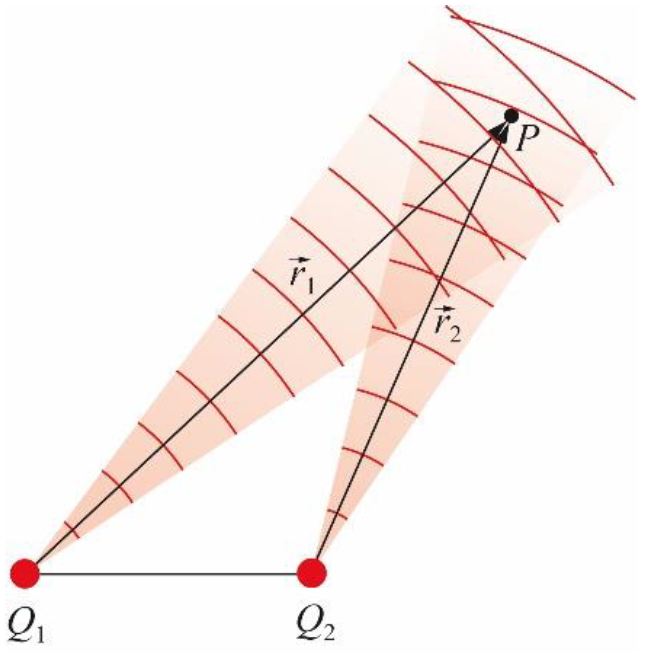
\includegraphics[width=0.7\linewidth]{Bilder/Wellen-Optik/interferenz} \\
\end{minipage}
\hfill
\begin{minipage}{0.48\linewidth}
$$ \xi_1 = A \cdot \sin(\omega \, t - k \, r_1) $$

$$ \xi_2 = A \cdot \sin(\omega \, t - k \, r_2) $$
\end{minipage}

$$ \boxed{ \xi = 2 \, A \cdot \sin \left( \omega \, t - \frac{k (r_1 + r_2)}{2} \right) \,  \cos \left( k \frac{\Delta r}{2}  \right) } $$

$\Rightarrow$ Der $\cos$-Term hängt nur vom Ort ab! \\
$\Rightarrow$ Es gibt \textbf{Orte}, an denen Welle sich auslöscht!

% \vfill\null
% \columnbreak




\subsection{Kohärenz}

Zwei Wellen werden als kohärent bezeichnet, wenn eine \textbf{feste Phasendifferenz} zwischen den beiden Wellen besteht. \\
\vspace{0.2cm}
Kohärenz ist eine \textbf{Vorbedingung}, damit sich eine \textbf{Interferenz} bilden kann. \\
\vspace{0.2cm}
\textbf{Kohärenzlänge} ist der \textbf{maximale Streckenunterschied}, den zwei Wellen haben dürfen, damit eine \textbf{(stabile) Interferenz} beobachtet werden kann.


\subsection{Reflexion und Transmission}


\subsubsection{Verhalten von Wellem an Grenzflächen von zwei Medien}

Ein Teil der Welle wird reflektiert und ein Teil wird transmittiert \\

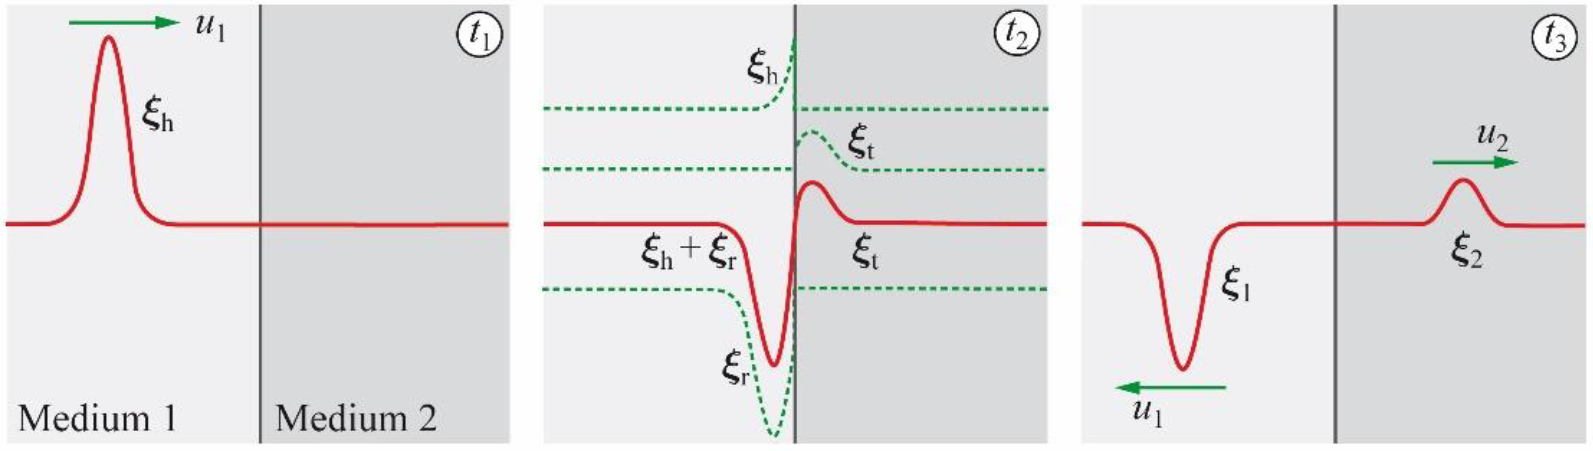
\includegraphics[width=0.95\linewidth]{Bilder/Wellen-Optik/reflexion_transmission} \\

\vspace{0.2cm}

\textbf{Physikalische Bedingung}\\
Stetigkeit der Wellenfunktion und der Ableitung an der Grenzfläche

$$ \xi_1(0) = \xi_2(0) \qquad \dot{\xi}_1(0) = \dot{\xi}_2(0) $$




\subsubsection{Intensität von Reflexion und Transmission}\label{Reflexionskoeffizient}

\begin{minipage}{0.48\linewidth}
	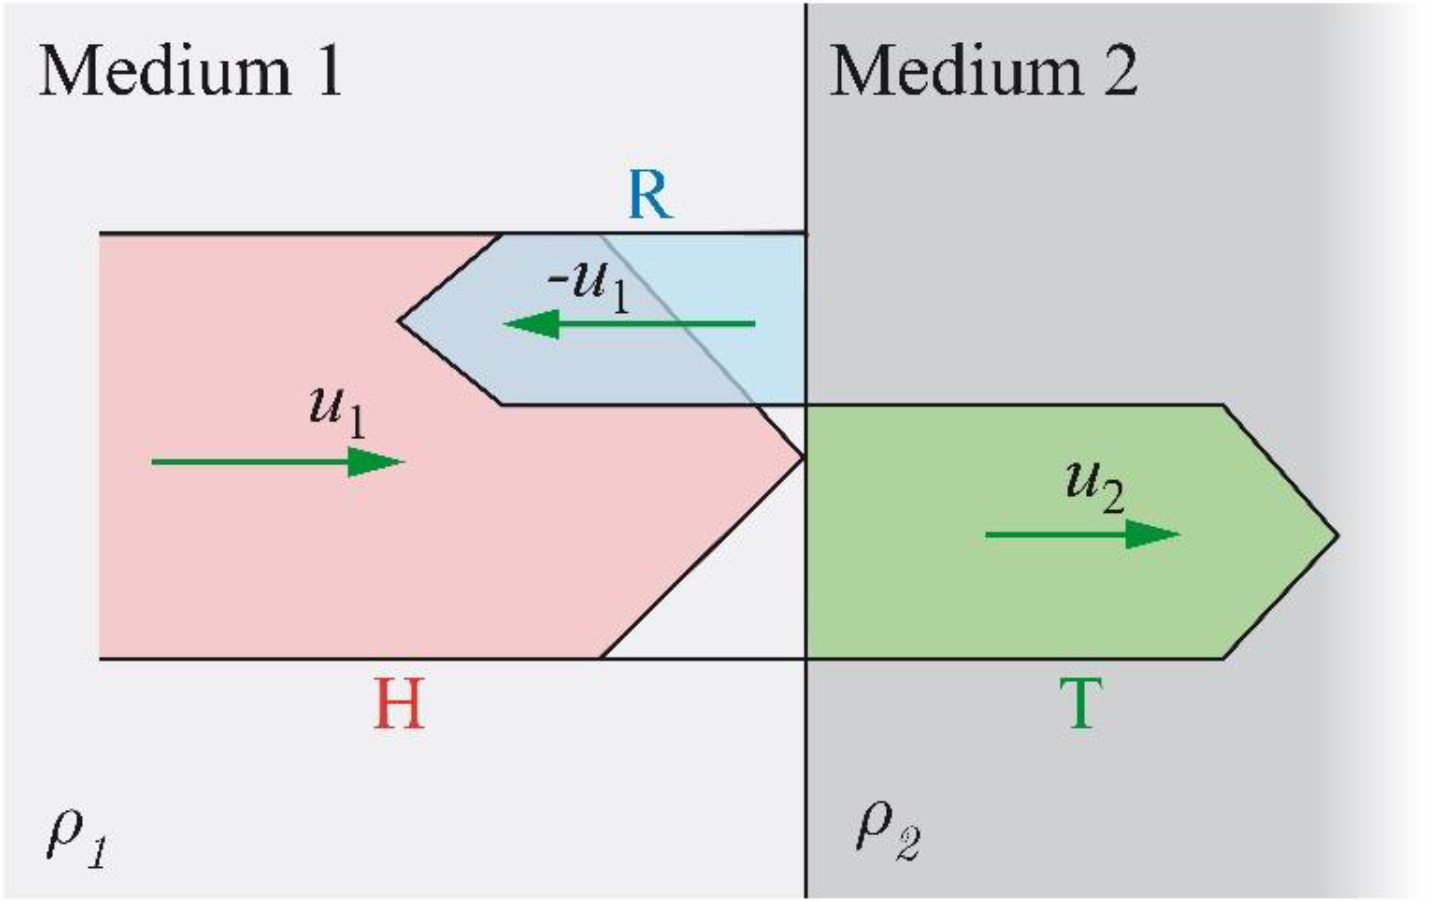
\includegraphics[width=0.9\linewidth]{Bilder/Wellen-Optik/reflexionskoeffizient_transmissionskoeffizient} \\
\end{minipage}
\hfill
\begin{minipage}{0.48\linewidth}
	$$ \boxed{ R = \left(  \frac{Z_1 - Z_2}{Z_1 + Z_2}  \right)^2  }  \quad \boxed{ T = \frac{ 4 \cdot Z_1 \cdot Z_2}{(Z_1 + Z_2)^2}   }$$
	$$ \boxed{ \sqrt{R} = \frac{Z_1 - Z_2}{Z_1 + Z_2} = \frac{u_R}{u_H} = \frac{A_R}{A_H} = \frac{p_R}{p_H} = ...} $$

	$$ \boxed{ \frac{2 \cdot Z_2}{(Z_1 + Z_2)}  = \frac{u_T}{u_H} = \frac{A_T}{A_H} = \frac{p_T}{p_H} = ... } $$
\end{minipage}

\vspace{0.2cm}


\renewcommand{\arraystretch}{1.1}
\begin{tabular}{clc}
$R$ & Reflexionskoeffizient  & $[R] = 1$ \\
$r$ & Amplitudenverhältnis  & $[r] = 1$ \\
$u_H$ & Geschw. hinlaufende Welle & $[u_H] = \frac{m}{s}$ \\
$u_R$ & Geschw. refl. Welle & $[u_R] = \frac{m}{s}$ \\
$u_T$ & Geschw. trans. Welle & $[u_T] = \frac{m}{s}$ \\
$p_H$ & Druck hinlaufende Welle & $[p_H] = Pa$ \\
$p_R$ & Druck refl. Welle & $[p_R] = Pa$ \\
$p_T$ & Druck trans. Welle & $[p_T] = Pa$ \\
$A_H$ & Ampl. hinlaufende Welle & $[A_H] = 1$ \\
$A_R$ & Ampl. refl. Welle & $[A_R] = 1$ \\
$A_T$ & Ampl. trans. Welle & $[A_R] = 1$ \\
$T$ & Transmissionskoeffizient & $[T] = 1 $ \\
$Z_n$ & Wellenwiderstand im Medium $n$ & $[Z] = \Ohm = \frac{\Pa}{\m / \s} = \frac{\N \, \s}{\m^3}$ \\
\end{tabular}
\renewcommand{\arraystretch}{1}



\subsubsection{Phasensprünge bei Reflexionen}

\begin{minipage}{0.4\linewidth}
	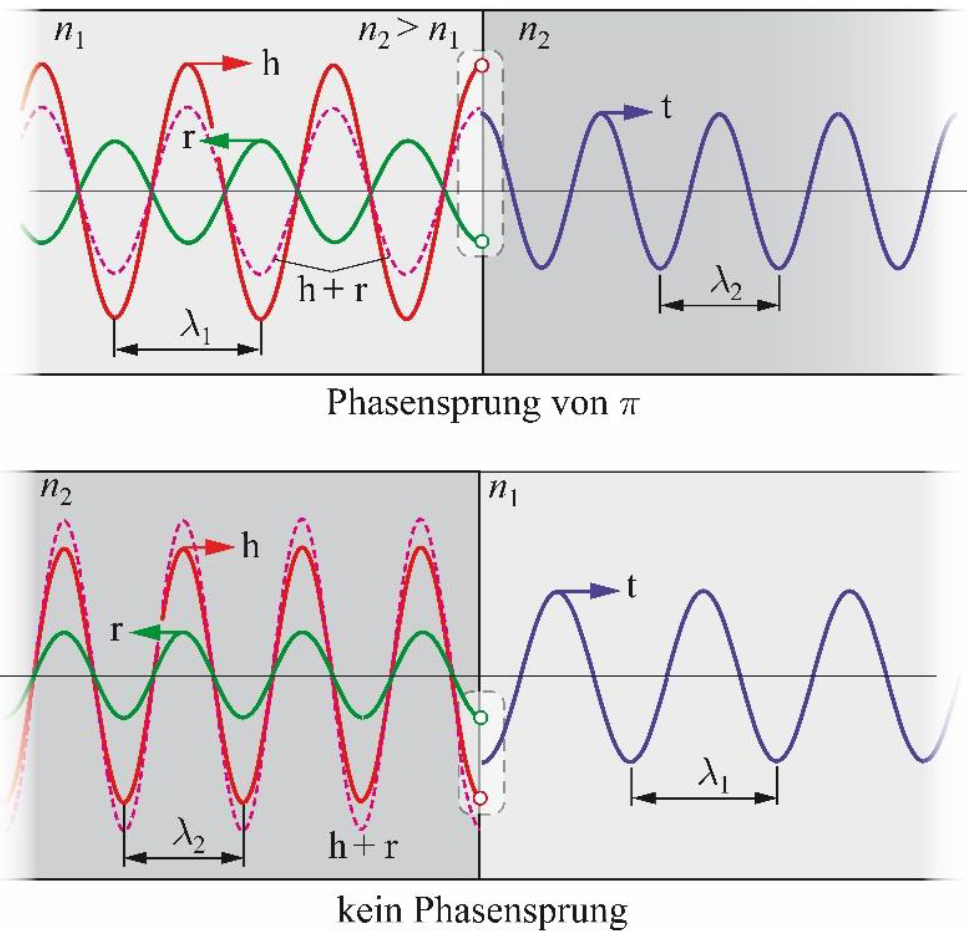
\includegraphics[width=0.9\linewidth]{Bilder/Wellen-Optik/reflexion_phasensprung} \\
\end{minipage}
\hfill
\begin{minipage}{0.58\linewidth}
	Reflexion an Material mit tieferer Wellenimpedanz\\
	$\Rightarrow$ \textbf{Phasensprung} \\
	(El. Impedanz : \(z\rightarrow 0\))\\

	dicht: $n_2 > n_1$ \\
	\textbf{kleinere} Wellengeschwindigkeit,\\
	\textbf{grösserer} Wellenwiderstand $Z$\\
	\vspace{0.2cm}

	Reflexion an Material mit höherer Wellenimpedanz\\
	$\Rightarrow$ \textbf{kein Phasensprung} \\
	(El. Impedanz : \(z\rightarrow \infty \))\\

\end{minipage}


\subsection{Anwendung: Elektromagnetische Wellen}

\subsubsection{Elektromagnetische Wellem in Doppelleiter}

\begin{minipage}{0.48\linewidth}
$$ \boxed{ u_r = \frac{Z_2 - Z_1}{Z_1 + Z_2} \, u_h } $$
\end{minipage}
\hfill
\begin{minipage}{0.48\linewidth}
$$ \boxed{ u_t = \frac{2 \, Z_2}{Z_1 + Z_2} \, u_h } $$
\end{minipage}


\begin{minipage}{0.48\linewidth}
$$ \boxed{ i_r = -\frac{Z_2 - Z_1}{Z_1 + Z_2} \, i_h } $$ \\
\end{minipage}
\hfill
\begin{minipage}{0.48\linewidth}
$$ \boxed{ i_t = \frac{2 \, Z_1}{Z_1 + Z_2} \, i_h } $$ \\
\end{minipage}

\textbf{Kabel mit kurzgeschlossenem Ende $\boldsymbol{Z_2 = 0}$} \\
\vspace{0.2cm}
\begin{minipage}{0.3\linewidth}
$$ u_r = - u_h $$ \\
\end{minipage}
\hfill
\begin{minipage}{0.68\linewidth}
$$ u_1 = u_h + u_r  = u_h - u_h = 0 $$ \\
\end{minipage}


\textbf{Kabel mit offenem Ende $\boldsymbol{Z_2 = \infty}$} \\
\vspace{0.2cm}
\begin{minipage}{0.3\linewidth}
$$ i_r = - i_h $$ 
\end{minipage}
\hfill
\begin{minipage}{0.68\linewidth}
$$ i_1 = i_r + i_h  = i_r - i_r = 0 $$  
\end{minipage}

\vspace{0.2cm}

\renewcommand{\arraystretch}{1.1}
\begin{tabular}{clc}
$u_r$ & Reflektierte Spannung & $[u_r] = \V$ \\
$u_h$ & Eintreffende Spannung & $[u_h] = \V$ \\
$i_r$ & Reflektierter Strom & $[i_r] = \A$ \\
$i_h$ & Eintreffender Strom & $[i_h] = \A$ \\
$Z_n$ & Wellenwiderstand im Medium $n$ & $[Z] = \Ohm = \frac{\Pa}{\m / \s} = \frac{\N \, \s}{\m^3}$ \\
\end{tabular}
\renewcommand{\arraystretch}{1}




\subsubsection{Elektromagnetische Wellen in homogenem Milieu}

$$ \boxed{ Z = \frac{E}{H} = \sqrt{ \frac{\mu_r \mu_0}{\varepsilon_r \varepsilon_0}} = \sqrt{\frac{\mu_r}{\varepsilon_r}} Z_0 = Z_0 \frac{c}{n}} \quad \boxed{ R = \left(  \frac{Z_1 - Z_2}{Z_1 + Z_2}  \right)^2 =  \left(  \frac{n_1 - n_2}{n_1 + n_2}  \right)^2 }$$


$$ \boxed{ E_{r0} = \frac{Z_2 - Z_1}{Z_1 + Z_2} E_{h0} } \quad \boxed{E_{t0} = \frac{2 \cdot Z_2}{Z_1 + Z_2} E_{h0}} $$

\renewcommand{\arraystretch}{1.1}
\begin{tabular}{clc}
$R$ & Reflexionskoeffizient  & $[R] = 1$ \\
$Z_n$ & Wellenwiderstand im Medium $n$ & $[Z] = \Ohm = \frac{\Pa}{\m / \s} = \frac{\N \, \s}{\m^3}$ \\
$\mu_r$ & Permeabilitätszahl & $[\mu_r] = 1$ \\
$\varepsilon$ & Dielektizitätszahl & $[\varepsilon_r] = 1$ \\
$n_n$ & Brechungsindex von Medium $n$ & $[n_1] = 1$ \\
\end{tabular}


\renewcommand{\arraystretch}{1.2}
\begin{tabular}{ll}
$\varepsilon_0$ & El. Feldkonstante $\varepsilon_0 = 8.854 \cdot 10^{-12} \, \frac{\A \, \s}{\V \, \m}$ \\
$\mu_0$ & Magn. Feldkonstante $\mu_0 = 4 \pi \cdot 10^{-7} \frac{\N}{\A^2}$\\
$Z_0$ & Wellenwiderstand Vakuum $Z_0 \approx 376.73 \, \Ohm$ \\
$c$ & Lichtgeschwindigkeit $c = 300 \cdot 10^6 \, \mathrm{\frac{m}{s}}$ \\ 
\end{tabular}
\renewcommand{\arraystretch}{1}


% \vfill\null
% \columnbreak



\section{Stehende Wellen}

\subsubsection{Terminologie}

Eine \textbf{stehende Welle} ist eine Welle, bei der Orte maximaler Auslenkung (oder minimaler Auslenkungen) sich
\textbf{nicht fortbewegen} 


\begin{itemize}
	\item Ort- und Zeitabhängigkeit sind separiert 
	\item Die Welle bewegt sich nicht im Raum ('Muster bleibt stehen') 
\end{itemize}



$$ \boxed{ \xi(x, t) = \xi_0 \cdot \cos(\omega t) \cdot \cos(k x) } $$

$\Rightarrow$ $\sin()$-Terme sind auch erlaubt!\\
\vspace{0.2cm}

Orte, wo die Welle für alle Zeit $= 0$ ist heissen \textbf{Wellenknoten} \\
$\Rightarrow$ \textbf{Zwei benachbarte Knoten sind $\boldsymbol{\frac{\lambda}{2}}$ auseinander}\\
\vspace{0.2cm}

Orte, wo die Welle eine maximale Auslenkung erreicht, heissen \textbf{Wellenbauch} \\
$\Rightarrow$ \textbf{Zwei benachbarte Bäuche sind $\boldsymbol{\frac{\lambda}{2}}$ auseinander}





\subsection{Entstehung von stehenden Wellen}

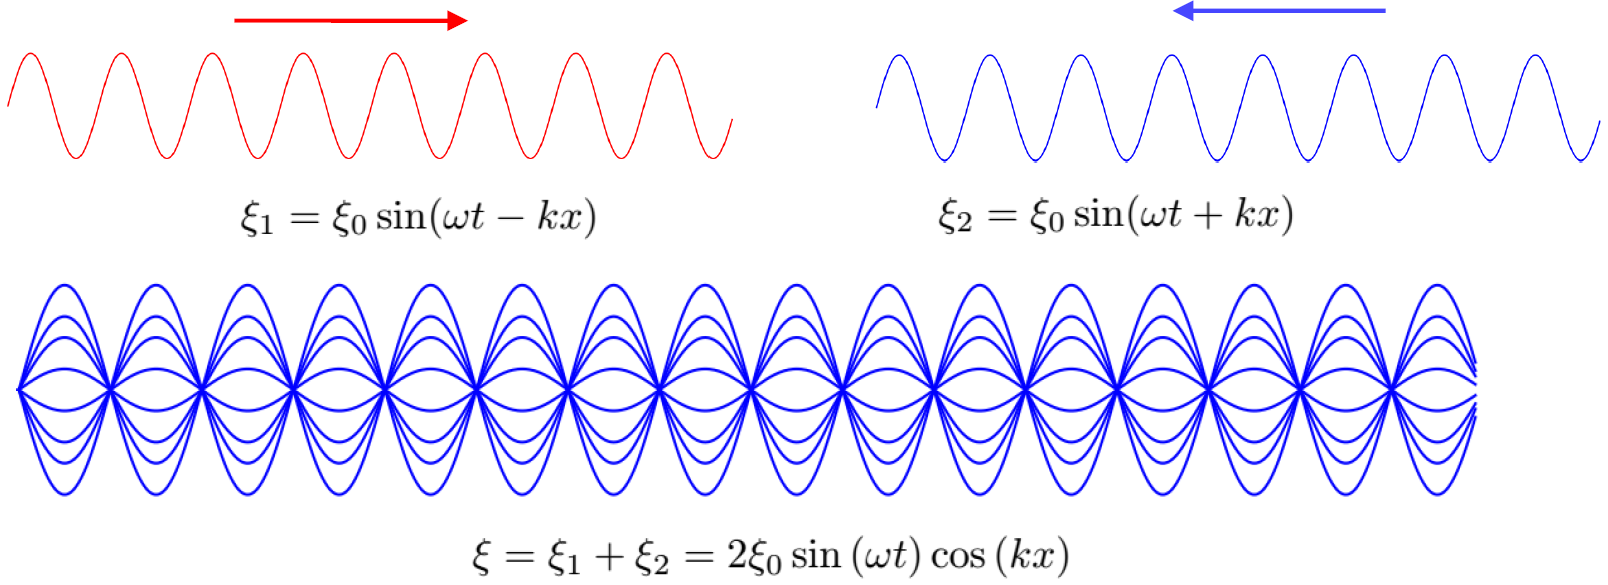
\includegraphics[width=0.9\linewidth]{Bilder/Wellen-Optik/stehende_wellen}



\subsection{Prinzip von Huygens}

\begin{minipage}{0.48\linewidth}
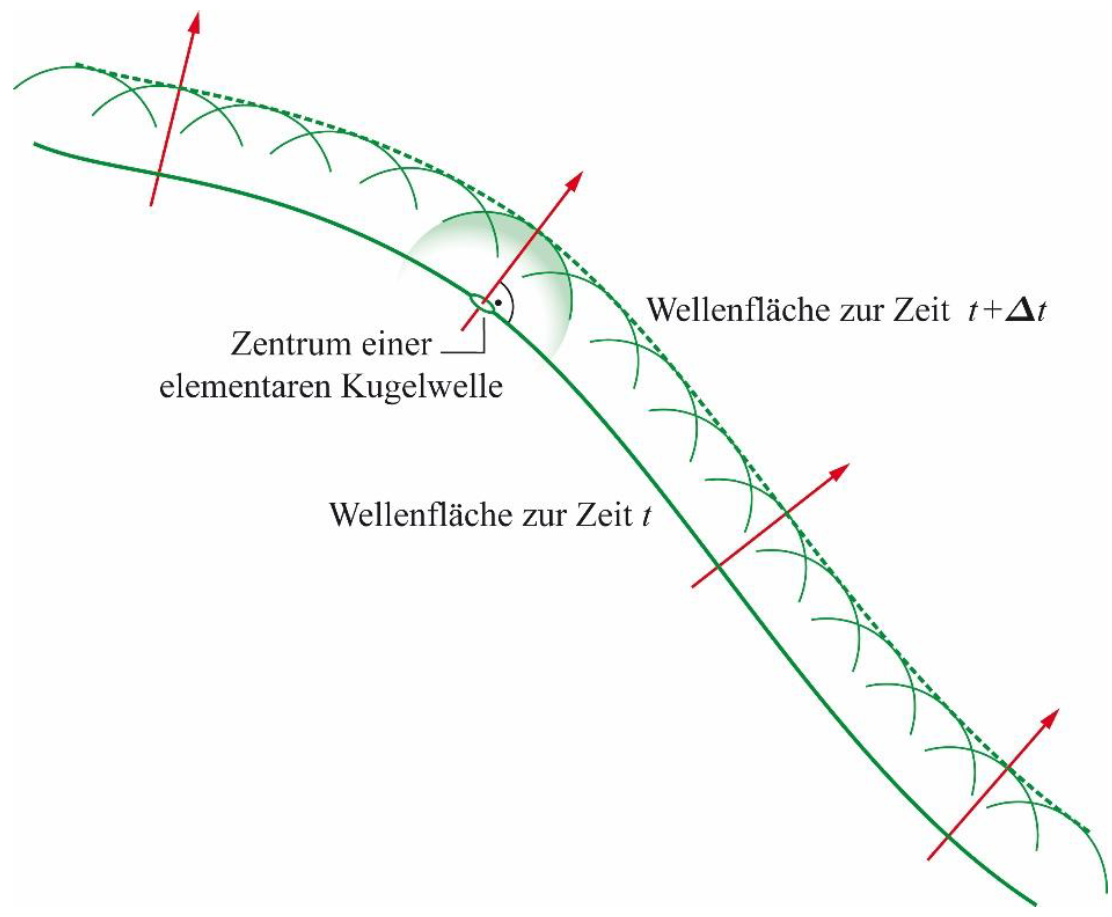
\includegraphics[width=0.9\linewidth]{Bilder/Wellen-Optik/huygens}
\end{minipage}
\hfill
\begin{minipage}{0.48\linewidth}
\raggedright
Jedes Flächenelement auf einer Wellenfläche kann als Zentrum einer Kugelwelle betrachtet\\
werden. \\
Die Wellenfläche zu einem späteren Zeitpunkt ist die Einhüllende all dieser Elementarwellen.
\end{minipage}

\subsection{Eigenschwingungen - 1D}

\begin{minipage}{0.3\linewidth}
$ \boxed{ f_n = \frac{n}{2 \, l} \cdot u = \frac{u}{\lambda_n} } $
\end{minipage}
\hfill
\begin{minipage}{0.66\linewidth}
$ \boxed{ \text{Auslenkung = 0: } k_n \cdot l = n \cdot \pi } $ \\
$ \boxed{ \text{Auslenkung max: } k_n \cdot l = \frac{\pi}{2} + n \cdot \pi  } $
\end{minipage}


\subsubsection{Saite}

\begin{itemize}
	\item Reflexion an einer Grenzfläche $\rightarrow$  Stehende Welle 
	\item Die stehende Welle muss in den vorhandenen Raum passen \\
		 $\rightarrow$ Geometrische Bedingung 
	\item \textbf{Knoten an beiden Enden} 
\end{itemize}



\begin{minipage}{0.48\linewidth}
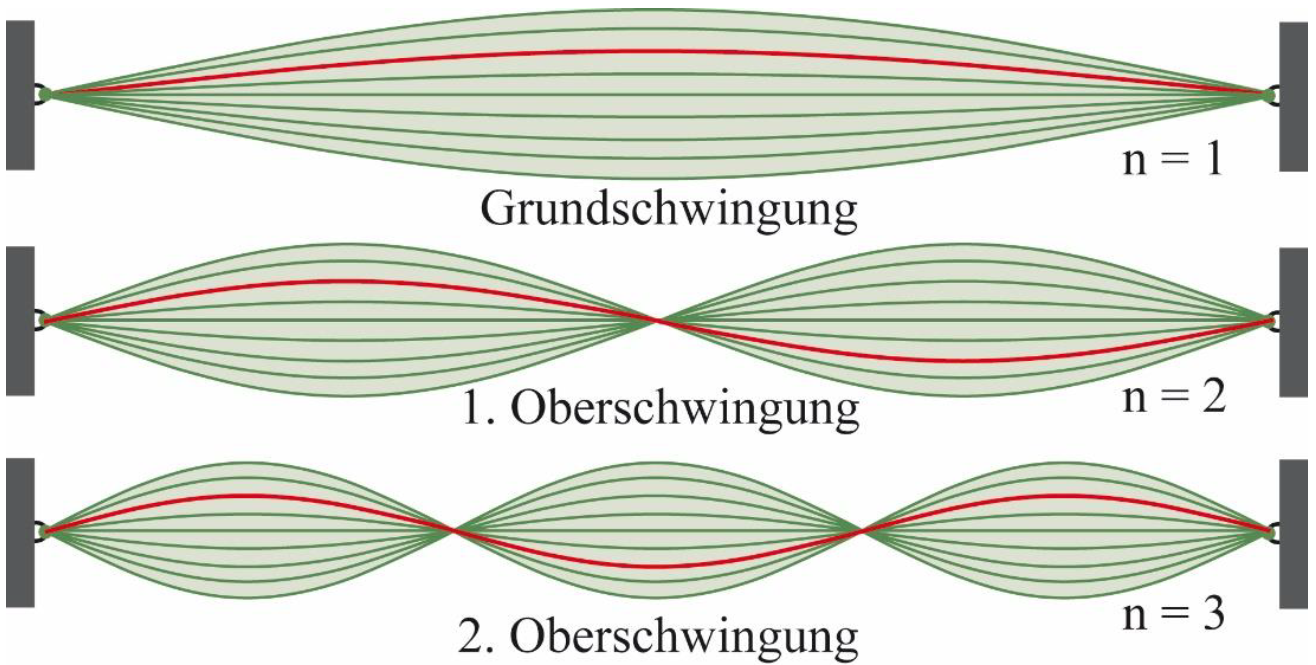
\includegraphics[width=0.98\linewidth]{Bilder/Wellen-Optik/saite} \\
\end{minipage}
\hfill
\begin{minipage}{0.48\linewidth}
$ \boxed{ \xi = \xi_0 \, \sin(\omega t) \cdot \sin(k x)  } $ \\

$ \boxed{ \text{Auslenkung = 0: } k_n \cdot l = n \cdot \pi } $ \\

$ \boxed{ f_n = \frac{u}{\lambda_n} = \frac{n}{2 \, l} \cdot u =  \frac{n}{2 \, l} \sqrt{\frac{F}{\rho \cdot A}} } $ \\
\end{minipage}

\vspace{0.2cm}

\renewcommand{\arraystretch}{1.1}
\begin{tabular}{clc}
$k_n$ & Wellenzahl & $[k_n] = \frac{1}{\m} $ \\
$l$ & Länge der Saite & $[l] = \m$ \\
$u$ & Wellengeschwindigkeit & $[u] \frac{\m}{\s}$ \\
$\lambda_n$ & Wellenlänge & $[\lambda_n]= \m$ \\
$n$ & Ganze Zahl & $[n] = 1$ \\
$\omega$ & Kreisfrequenz & $[\omega] = \frac{\rad}{\s}$ \\
$A$ & Querschnitt der Saite & $[A] = \m^2$
\end{tabular}



\subsubsection{Pfeifen}

\begin{minipage}{0.48\linewidth}
	\textbf{Offene Pfeife}\\
	Länge $l = \frac{\lambda}{2}$ \\

	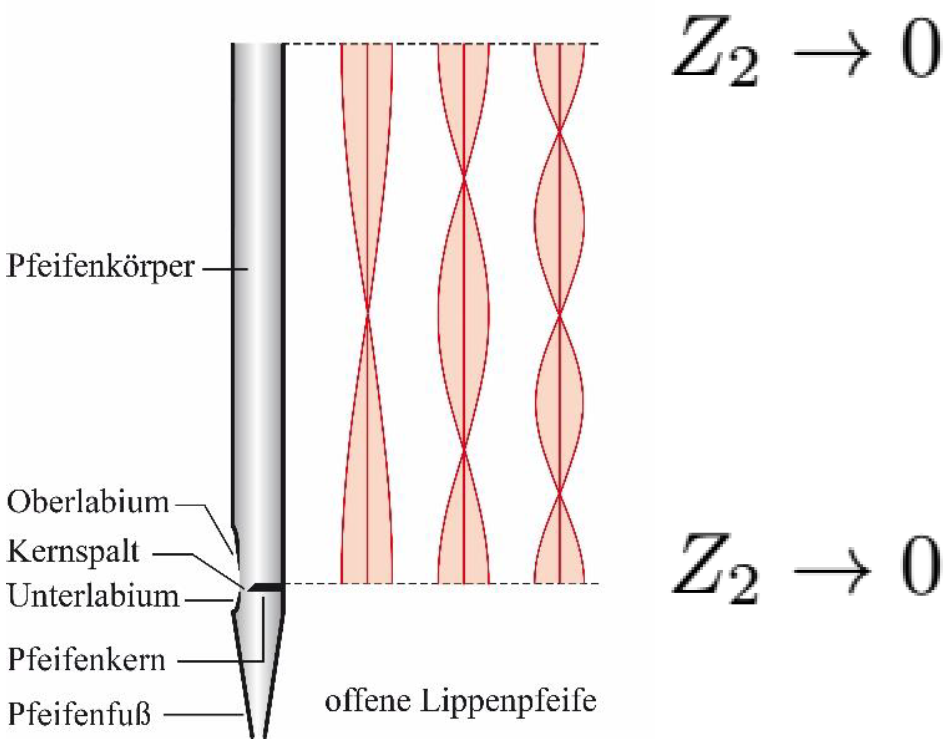
\includegraphics[width=0.8\linewidth]{Bilder/Wellen-Optik/offene_pfeiffe}\\

	Auslenkung an Enden: \\
	Wellenbauch \\
\end{minipage}
\hfill
\begin{minipage}{0.48\linewidth}
	\textbf{Gedackte Pfeife} \\
	Länge $l = \frac{\lambda}{4}$ \\

	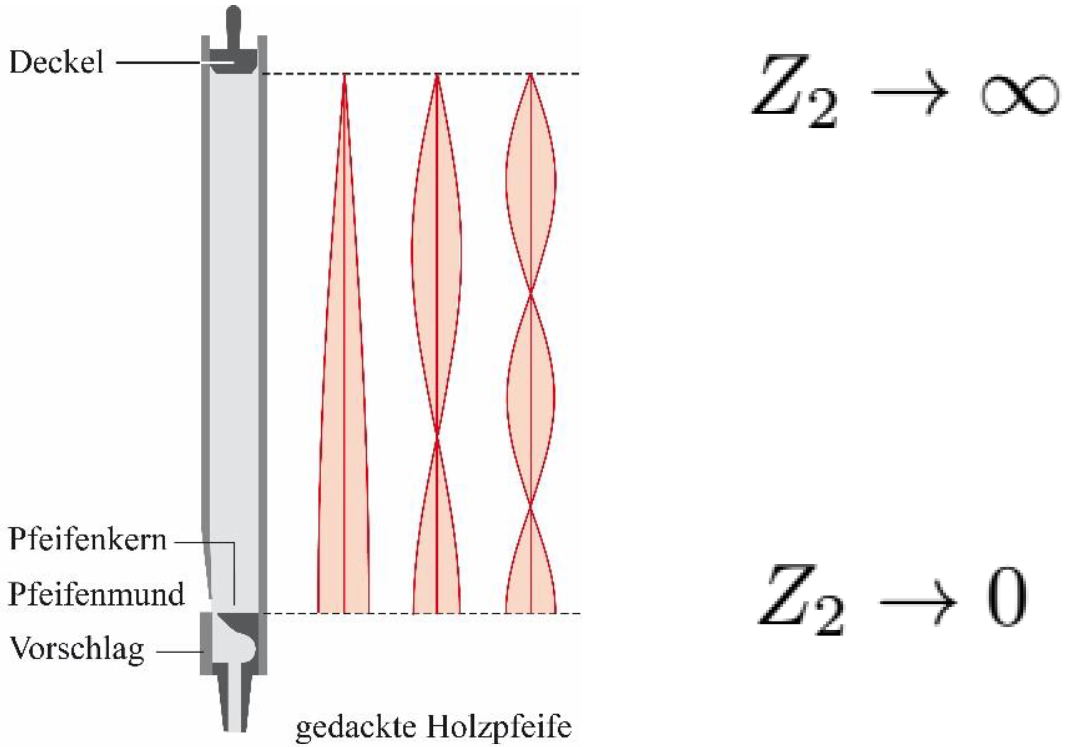
\includegraphics[width=0.85\linewidth]{Bilder/Wellen-Optik/gedackte_pfeiffe} \\

	Auslenkung offenes Ende: Wellenbauch \\
	Auslenkung gedacktes Ende: Knoten \\
	(max. Auslenkung) \\
\end{minipage}

\begin{center}
	$ \boxed{f_n = \underbrace{\frac{n}{2l}\sqrt{\frac{\varkappa R T}{M}}}_{\text{offen}}, \qquad f_n = \underbrace{\frac{2n+1}{4l}\sqrt{\frac{\varkappa R T}{M}}}_{\text{gedackt}}} $
\end{center}


\subsection{Eigenschwingungen - 2D}

\subsubsection{Rechteckige Membrane}


\begin{minipage}{0.3\linewidth}
	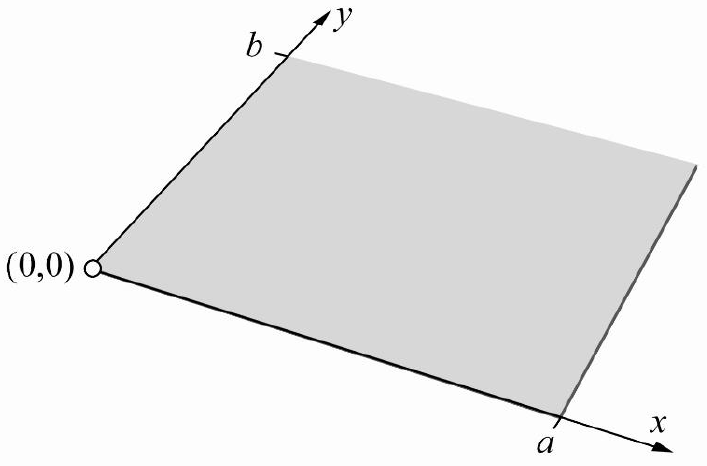
\includegraphics[width=0.98\linewidth]{Bilder/Wellen-Optik/membrane} \\
	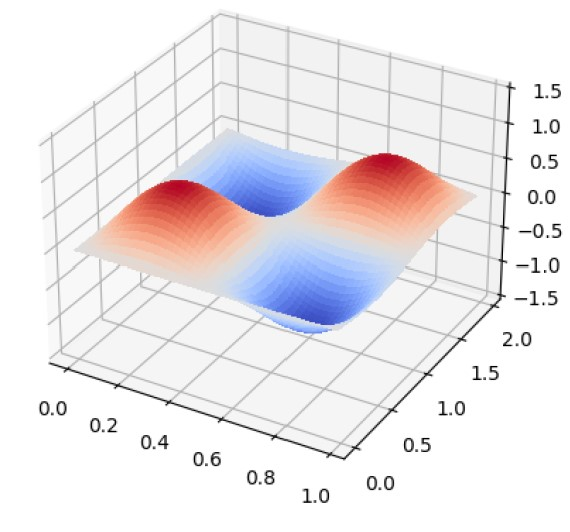
\includegraphics[width=0.98\linewidth]{Bilder/Wellen-Optik/membrane-3d.jpg} \\
\end{minipage}
\hfill
\begin{minipage}{0.68\linewidth}
	$$ \boxed{ \xi(x,y,t) = \xi_0 \, \sin(\omega t) \, \sin(k_x x) \, \sin(k_y y)  } $$

	$$ \boxed{ g(t)\frac{\partial^2f}{\partial x^2} + g(t)\frac{\partial^2f}{\partial y^2} = \frac{1}{u^2}f(x,y)g(t)\frac{\partial^2g}{\partial t^2} } $$

	$$ \boxed{ \text{Wellenvektor: } k = |\vec{k}| = \sqrt{k_x^2 + k_y^2}} $$

	$$ \boxed{ u^2 = \frac{\omega^2}{k^2}} $$
\end{minipage}

\textbf{Randbedingungen:} %\\
\begin{tabular}{l c c }
	Auslenkung = 0 &  $ \boxed{ k_x = \frac{n \, \pi}{a} }$ & $ \boxed{ k_y = \frac{m \, \pi}{b} }$
\end{tabular} 

\begin{minipage}{0.45\linewidth}
	\begin{tabular}{clc}
		$u$ & Wellengeschwindigkeit & $[u] = \frac{\m}{\s}$ \\
		$m$ & Ganze Zahl & $[m] = 1$ \\
		$n$ & Ganze Zahl & $[n] = 1$ \\
		$\omega$ & Kreisfrequenz & $[\omega] = \frac{\rad}{\s}$ \\
		$k_{...}$ & Wellenzahl & $[k_{...}] = \frac{1}{\m} $ \\
		$a,b$ & Seitenlänge Membran & $[a,b] = \m$ \\
		$A$ & Querschnitt der Membrane & $[A] = \m^2$
	\end{tabular}
\end{minipage}
\hfill
\begin{minipage}{0.45\linewidth}
	$$ \boxed{f_{mn} = \frac{1}{2}\sqrt{\frac{F}{\rho A}}\sqrt{\frac{m^2}{a^2} + \frac{n^2}{b^2}}} $$
\end{minipage}



\section{Beugung}

\subsubsection{Terminologie}

Die \textbf{Richtungsänderungen} der Wellenausbreitung in einem homogenen Medium durch \textbf{Hindernisse} wird als \textbf{Beugung (Diffraktion)} bezeichnet. \\
\begin{itemize}
	\item Das Hindernis kann eine Kante, ein Spalt oder ein kleines \\
	Objekt sein sein 
	\item Beugung tritt auf, wenn das \textbf{Hindernis} von \textbf{ähnlicher}\\
	\textbf{Grösse} ist, wie die \textbf{Wellenlänge} 
\end{itemize}


$\Rightarrow$ \textbf{Beugung tritt auf, wenn eine Welle limitiert wird!} \\
\vspace{0.2cm}

Dies gilt insbesondere für: \\
Spalt, Kante, Loch (Pinhole), Objektiv-Öffnung


\subsection{Beugung - Spalt}

\subsubsection{Beschreibung Setup}\label{Beschreibung Setup}

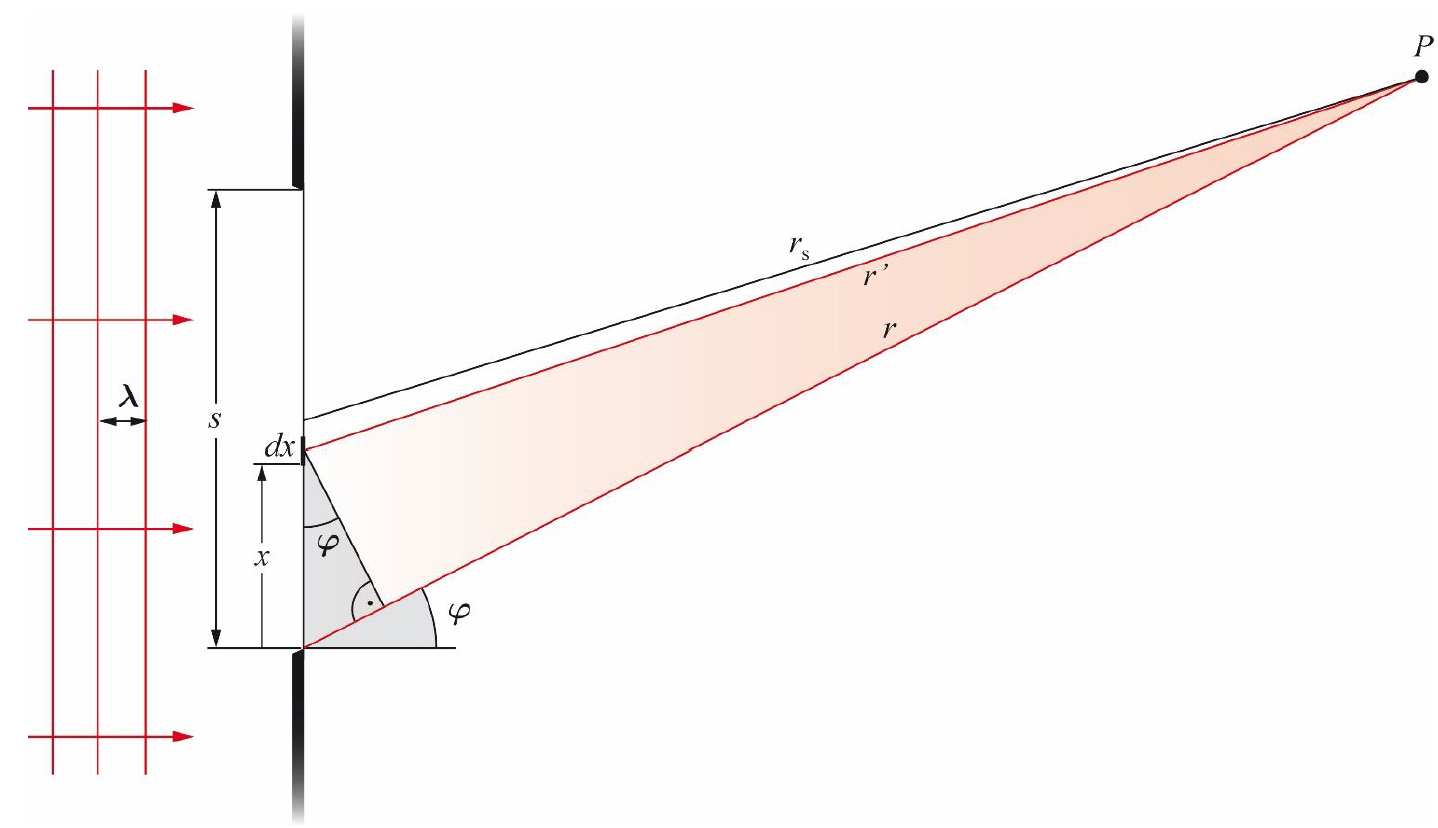
\includegraphics[width=0.7\linewidth]{Bilder/Wellen-Optik/beugung_spalt} 


\subsubsection{Intensität nach dem Spalt}\label{Spalt-Intensitaet}


\begin{minipage}{0.58\linewidth}
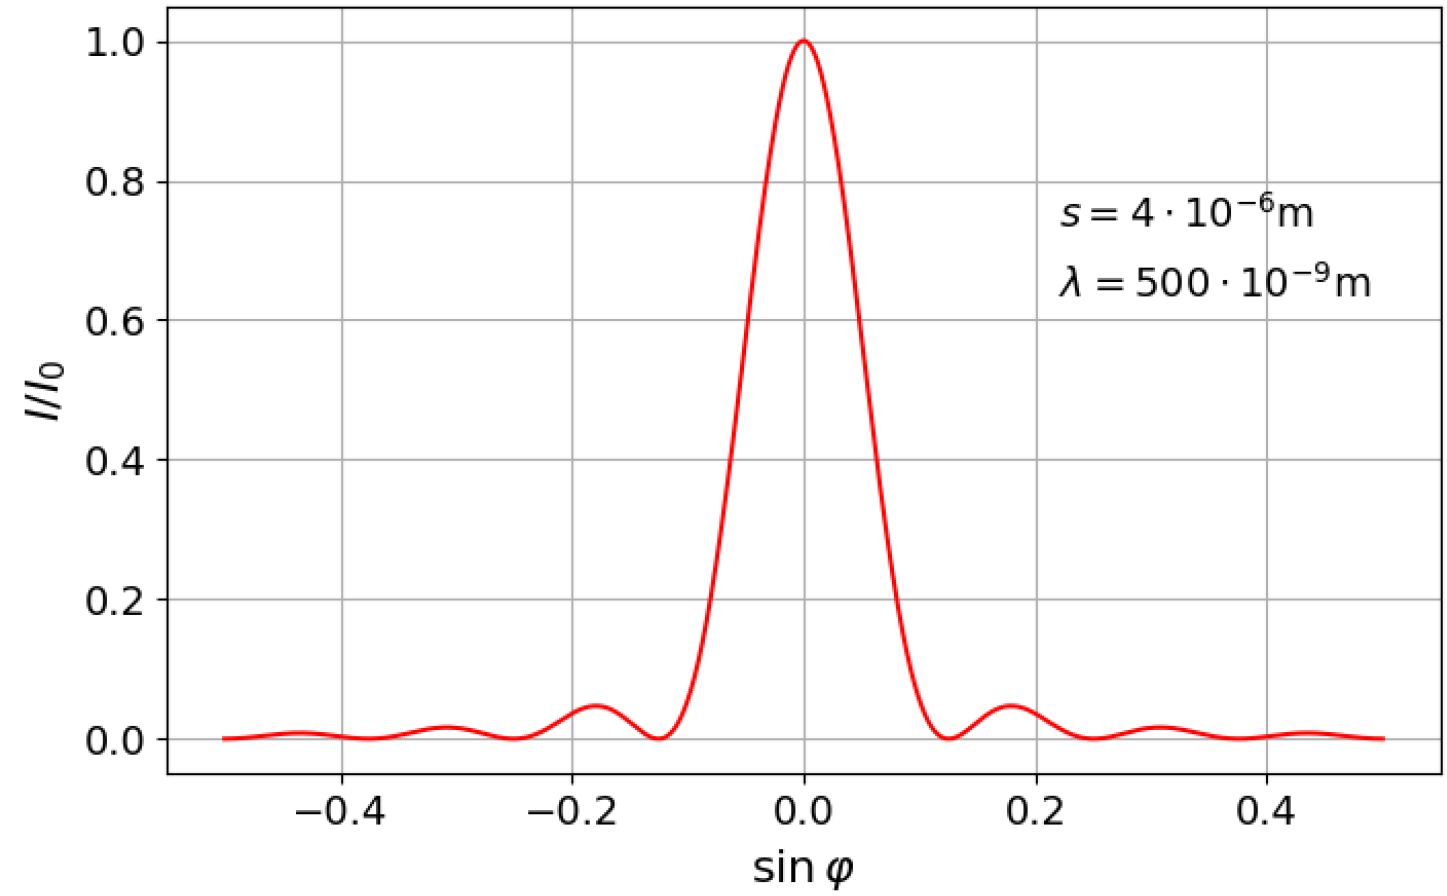
\includegraphics[width=0.98\linewidth]{Bilder/Wellen-Optik/beugung_spalt_intensitaet} \\
\end{minipage}
\hfill
\begin{minipage}{0.4\linewidth}
$$ \boxed{ I_s \varpropto \frac{A^2}{r^2} \frac{\sin^2\Big( \frac{k \cdot s \cdot \sin(\varphi)}{2} \Big) }{\Big( \frac{k \cdot s \cdot \sin(\varphi)}{2} \Big)^2 } } $$


\textbf{Minima der Intensität} 

$$ \boxed{ \sin(\varphi) = n \, \frac{\lambda}{s}} $$ \\
\end{minipage}



\renewcommand{\arraystretch}{1.1}
\begin{tabular}{clc}
$I_s$ & Intensität & $[I_s] = \frac{W}{\m^2}$ \\
$s$ & Länge des Spalts & $[s] = \m$ \\
$\lambda$ & Wellenlänge & $[\lambda]= \m$ \\
$n$ & Ordnung (typ. 1) & $[n] = 1$ \\
$A$ & Amplitude & $[A]$ \\
$r$ & siehe Bild Abschnitt \ref{Beschreibung Setup} & $[r] = \m$ \\
$\varphi$ & Einfallswinkel der Welle zum Spalt & $[\varphi] =$° \\
 & \textcolor{blue}{Hinweis: Oft muss gegebenes $\varphi$ durch 2} & \\
 & \textcolor{blue}{geteilt werden!} \\
\end{tabular}
\renewcommand{\arraystretch}{1}

% \vfill\null
% \columnbreak


\subsection{Beugung - Runde Öffnung (Pinhole)}

\begin{minipage}{0.48\linewidth}
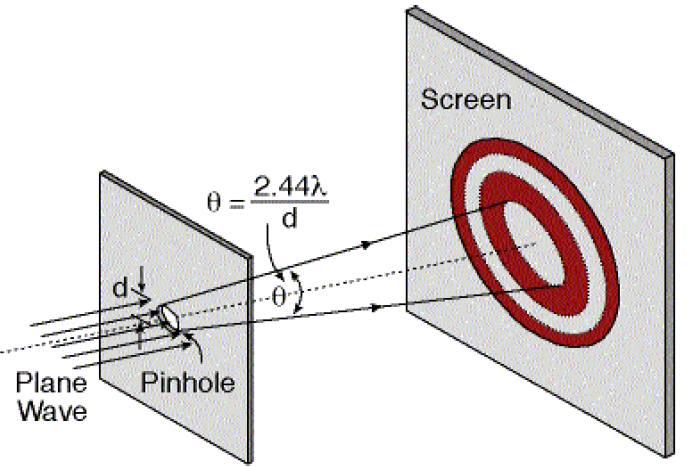
\includegraphics[width=0.98\linewidth]{Bilder/Wellen-Optik/beugung_loch} \\
\end{minipage}
\hfill
\begin{minipage}{0.48\linewidth}
\textbf{Nullstelle erster Ordnung:} 

$$ \boxed{ \sin(\varphi) = 1.22 \frac{\lambda}{D} } $$ 
\end{minipage}


\renewcommand{\arraystretch}{1.1}
\begin{tabular}{clc}
$\lambda$ & Wellenlänge & $[\lambda]= \m$ \\
$D$ & Loch-Durchmesser & $[D] = \m$
\end{tabular}
\renewcommand{\arraystretch}{1}



\subsection{Beugung - Gitter} % TODO: Formeln aus Buch eintragen

\subsubsection{Beschreibung Setup}
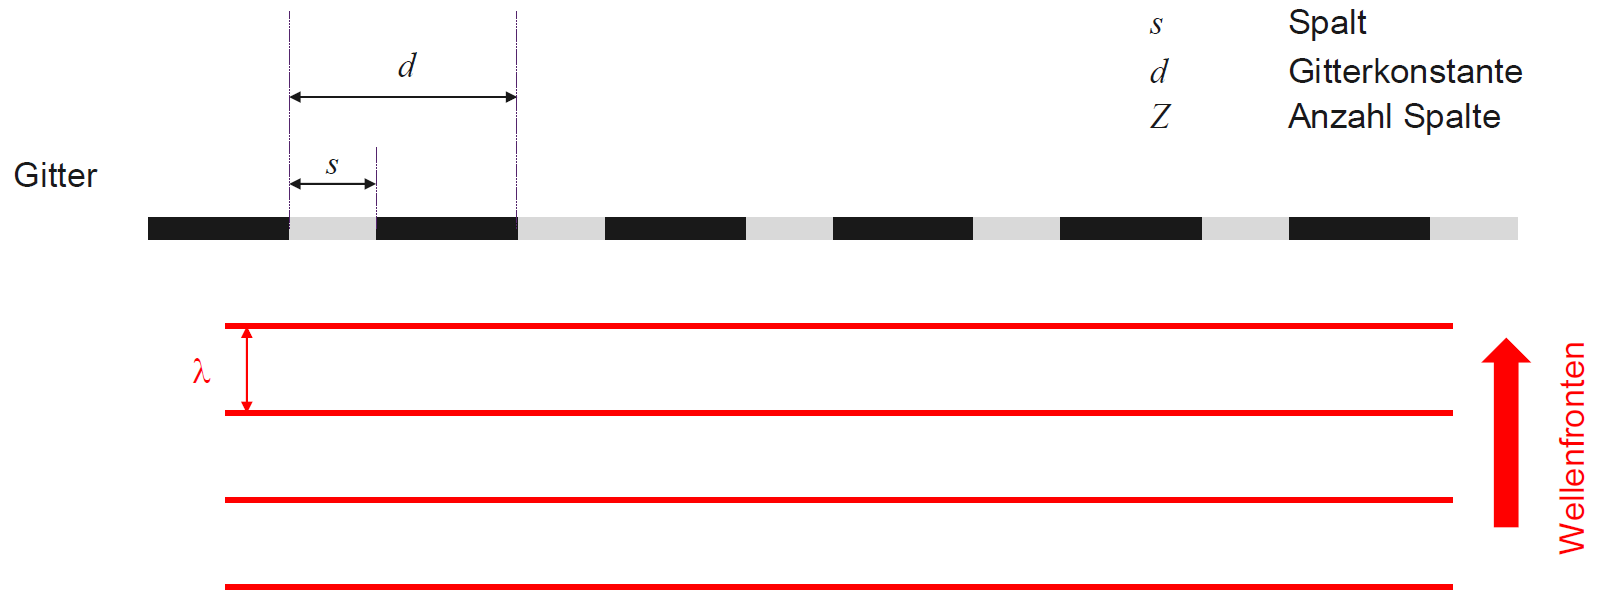
\includegraphics[width=0.9\linewidth]{Bilder/Wellen-Optik/beugung_gitter} 


\subsubsection{Intensität nach dem Gitter}

$$ \boxed{ I_G = \frac{A^2}{r^2} \textcolor{red}{A_s^2} \, \textcolor{green}{B^2} }$$


% \begin{minipage}{0.48\linewidth}
% $$\textcolor{blue}{A_s^2(\varphi) = \frac{\sin^2\Big( \frac{k \cdot s \cdot \sin(\varphi)}{2} \Big) }{\Big( \frac{k \cdot s \cdot \sin(\varphi)}{2} \Big) } } $$
% \end{minipage}
% \hfill
% \begin{minipage}{0.48\linewidth}
% $$ \textcolor{orange}{B^2(\varphi) = \frac{\sin^2 \Big( Z  \frac{k \cdot d \cdot \sin(\varphi)}{2} \Big) }{\Big( \frac{k \cdot d \cdot \sin(\varphi)}{2} \Big) }  }$$
% \end{minipage}


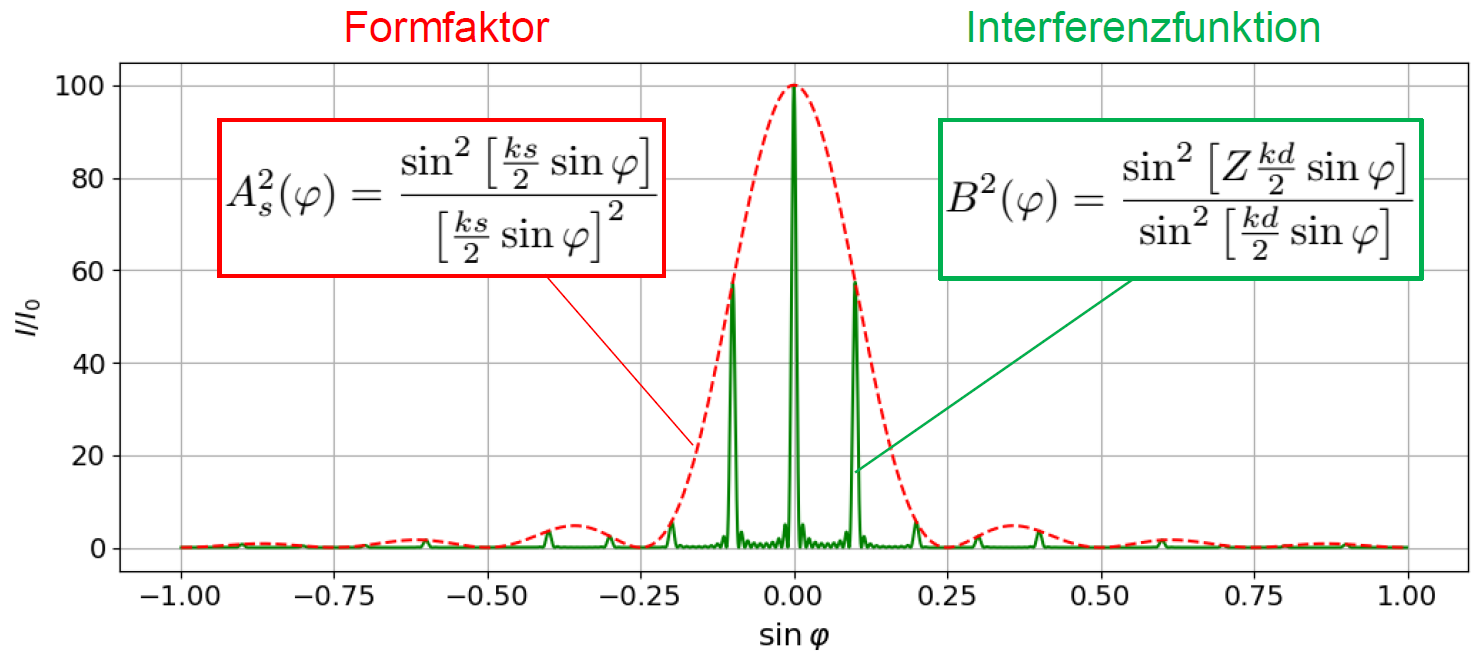
\includegraphics[width=0.9\linewidth]{Bilder/Wellen-Optik/beugung_gitter_intensitaet} \\
\vspace{0.2cm} 
\renewcommand{\arraystretch}{1.2}
\begin{tabular}{ll}
$A_s^2(\varphi)$ & hat Nullstellen bei $n \, \frac{\lambda}{s}$ (hängt von $s$ ab), gleiches $A_s$ wie in \ref{Spalt-Intensitaet} \\
$B^2(\varphi)$ & hat Hauptmaxima bei $n \, \frac{\lambda}{d}$ und $Z - 2$ Nebenmaxima\\
& dazwischen (hängt von $Z$ und $d$ ab)\\
\end{tabular}
\renewcommand{\arraystretch}{1}


\vspace{0.2cm}

\renewcommand{\arraystretch}{1.3}
\begin{tabular}{clc}
$I_G$ & Intensität nach Gitter & $[I_G] = \frac{W}{\m^2}$ \\
$k$ & Wellenzahl & $[k] = \frac{1}{\m}$ \\
$s$ & Spalt & $[s] = \m$ \\
$d$ & Gitterkonstante & $[d] = \m$ \\
$Z$ & Anzahl der Spalten & $[Z] = 1$
\end{tabular}
\renewcommand{\arraystretch}{1}

% \vfill\null
% \columnbreak


\subsubsection{Auflösungsvermögen}

Verschiedene Wellenlängen können getrennt (aufgelöst) werden \\


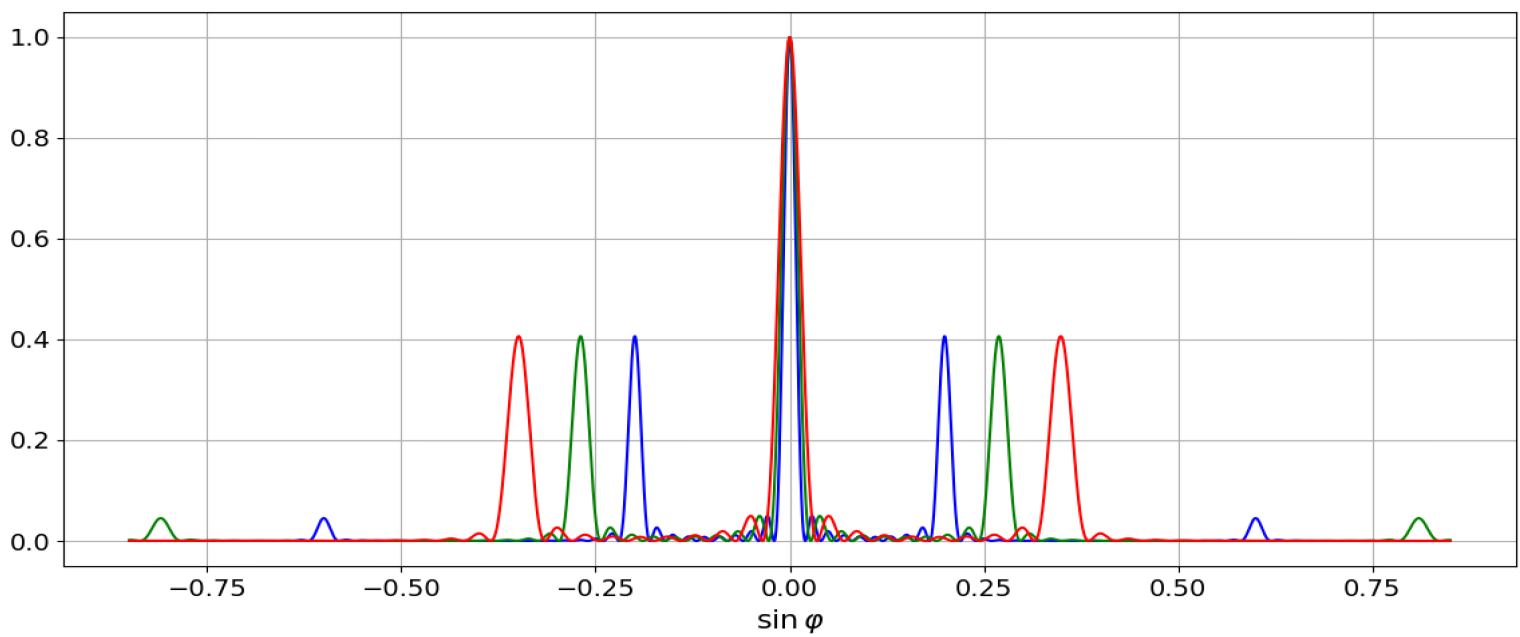
\includegraphics[width=0.9\linewidth]{Bilder/Wellen-Optik/aufloesungsvermoegen} \\

\vspace{0.2cm}

\textbf{Kriterium}\\

Zwei Wellenlängen werden gerade
noch aufgelöst, wenn das
Hauptmaximum von $\lambda_2$ mit dem Minimum von $\lambda_1$ zusammenfällt

$$ \boxed{ \frac{\lambda}{\Delta \lambda} = n \, Z } $$


\renewcommand{\arraystretch}{1.3}
\begin{tabular}{clc}
$\lambda$ & Wellenlänge & $[\lambda] = \m$ \\
$\Delta \lambda$ & Unterschied der Wellenlängen & $[ \Delta \lambda] = \m$ \\
$n$ & Ordnung der Beugung (typ. 1) & $[n] = 1$ \\
$Z$ & Anzahl der Spalten & $[Z] = 1$ 
\end{tabular}
\renewcommand{\arraystretch}{1}




\subsection{Babinet-Prinzip}

\begin{minipage}{0.48\linewidth}
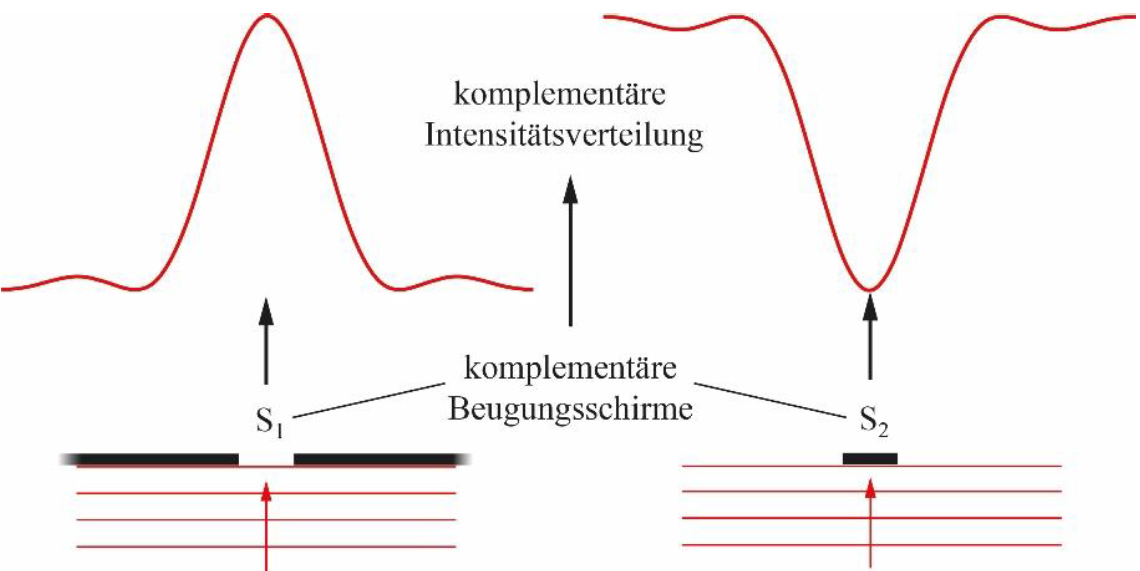
\includegraphics[width=0.98\linewidth]{Bilder/Wellen-Optik/babinet_prinzip} \\
\end{minipage}
\hfill
\begin{minipage}{0.48\linewidth}

Ausserhalb des Bereichs \\
geometrisch-optischer Abbildung\\
produzieren komplementäre\\
Beugungsschirme gleiche \\
Beugungsbilder
\end{minipage}





\section{Akustik}

\subsubsection{Terminologie}

\textbf{Ton}\\
Eine harmonische Schallwelle wird als \textbf{Ton} bezeichnet. \\
Ein (reiner) Ton entspricht also einer \textbf{Schallschwingung}, die \textbf{eine
einzige Frequenz} enthält. \\
\vspace{0.2cm}

\textbf{Klang} \\
Eine \textbf{Überlagerung} von harmonischen Schwingungen, deren
\textbf{Frequenzen} in einem \textbf{ganzzahligen Verhältnis} zur tiefsten
Frequenz, zur Frequenz des \textbf{Grundtons}, stehen, wird \textbf{Klang}
genannt. \\
\vspace{0.2cm}

\textbf{Geräusch} \\
Bei einem \textbf{Geräusch} besteht das Frequenzspektrum nicht mehr
aus einzelnen diskreten Linien, sondern weist in einem
bestimmten Frequenzbereich eine  \textbf{kontinuierliche Verteilung} auf. \\




\subsection{Pegel}\label{Pegel}

\begin{minipage}{0.48\linewidth}
\center{\textbf{'Einheit': Bel}} 
$$ \boxed{ \text{Pegel} = \log \Big( \frac{x}{b_0} \Big) } $$
$$ \boxed{ x = b_0 \cdot 10^{\text{Pegel} } } $$ 

\end{minipage}
\hfill
\begin{minipage}{0.48\linewidth}
\center{\textbf{'Einheit': Dezibel}}
$$ \boxed{ \text{Pegel} = 10 \cdot \log \Big( \frac{x}{b_0} \Big) } $$ 
$$ \boxed{ x = b_0 \cdot 10^{\Big( \frac{\text{Pegel}}{10} \Big) } } $$ \\
\end{minipage}

\renewcommand{\arraystretch}{1.3}
\begin{tabular}{clc}
Pegel & Dimensionslose Grösse & $[\text{Pegel}] =  1$ \\
$x$ & Zu vergleichende Grösse & $[x]$ \\
$b_0$ & Basisgrösse & $[b_0] = [x]$ \\
\end{tabular}
\renewcommand{\arraystretch}{1}

\raggedright



\subsection{Schallintensität}

\begin{minipage}{0.28\linewidth}
	$$ \boxed{ L_I = 10 \cdot \log \left( \frac{I}{I_0} \right) } $$ 
\end{minipage}
\hfill
\begin{minipage}{0.40\linewidth}
	$$ \boxed{I = \frac{1}{2}\rho v_0^2 u = \frac{\Delta p_0^2}{2 \rho u} }$$ 
\end{minipage}
\hfill
\begin{minipage}{0.28\linewidth}
	$$ \boxed{ p_{eff} = \frac{\Delta p_0}{\sqrt{2}} } $$ 
\end{minipage}

\begin{minipage}{0.28\linewidth}
	$$ \boxed{ L_p = 20 \cdot \log \left( \frac{p_{eff}}{p_{eff0}} \right) } $$ 
\end{minipage}
\hfill
\begin{minipage}{0.28\linewidth}
	$$ \boxed{ L_P = 10 \cdot log \left(\frac{P}{P_0}\right)} $$ 
\end{minipage}

\renewcommand{\arraystretch}{1.3}
\begin{tabular}{clc}
	$L_I$ & Schallintensitätspegel & $[L_I] = \dB$ \\
	$I$ & Intensität & $[I] = \frac{\W}{\m^2}$\\
	$I_0$ & Bezugsintensität  & $I_0 = 10^{-12} \frac{\W}{\m^2}$ \\
	$L_p$ & Schalldruckpegel & $[L_p] = \dB$ \\
	$p_{eff}$ & Schalldruck (Effektivwert) & $[p_{eff}] = \Pa$ \\
	$p_{eff0}$ & Bezugsschalldruck & $p_{eff0} = 2 \cdot 10^{-5} \Pa$ \\
	$L_P$ & Schallleistungspegel & $[L_P] = \dB$ \\
	$P$ & Schallleistung & $[P] = \W$ \\
	$P_0$ & Bezugsschallleistung & $P_0 = 10^{-12} \W$ \\
	$\Delta p_0$ & Druckamplitude & $[\Delta p_0] = \Pa$ \\
\end{tabular}
\renewcommand{\arraystretch}{1}

\subsection{Intensität bei Kugelwellen}
\begin{tabular}{lll}
					 & \textbf{ohne Dämpfung} & \textbf{mit Dämpfung} \\
	Energieerhaltung & $ \boxed{ I(r) = \frac{P}{4 \, \pi \, r^2} }$ & $ \boxed{ I(r) = \frac{P}{4 \, \pi \, r^2} \, \e^{- \alpha r}}$\\

	Verhältnis 		 & $\boxed{ \frac{I_2}{I_1} = \frac{r_1^2}{r_2^2} }$ & $\boxed{ \frac{I_2}{I_1} = \frac{r_1^2}{r_2^2} \, \e^{- \alpha (r_2 - r_1)} }$ \\

	Pegel 			 & $\boxed{ L_2 = L_1 - 20 \cdot \log \left( \frac{r_2}{r_1} \right)}$ & $\boxed{ L_2 = L_1 - 20 \cdot \log \left( \frac{r_2}{r_1} \right) - K (r_2 - r_1)  }$\\
\end{tabular}

\begin{tabular}{clc}
	$I(r)$ & Intensität & $[I(r)] = \frac{\W}{\m^2}$ \\
	$P$ & Leistung & $[P] = \W$ \\
	$r_i$ & Abstand (Radius) zum Wellenursprung & $[r_i] = \m^2$\\
	$L_i$ & Pegel & $[L_i] = \dB$ \\
	$\alpha$ & Absorptionsgrad ($\alpha = 1-R$, siehe \ref{Reflexionskoeffizient} ) & $[\alpha] = 1$ \\
	$K$ & Dämpfung & $[K] = \frac{\dB}{\m}$
\end{tabular}


\subsection{Verschiedene Schallquellen}

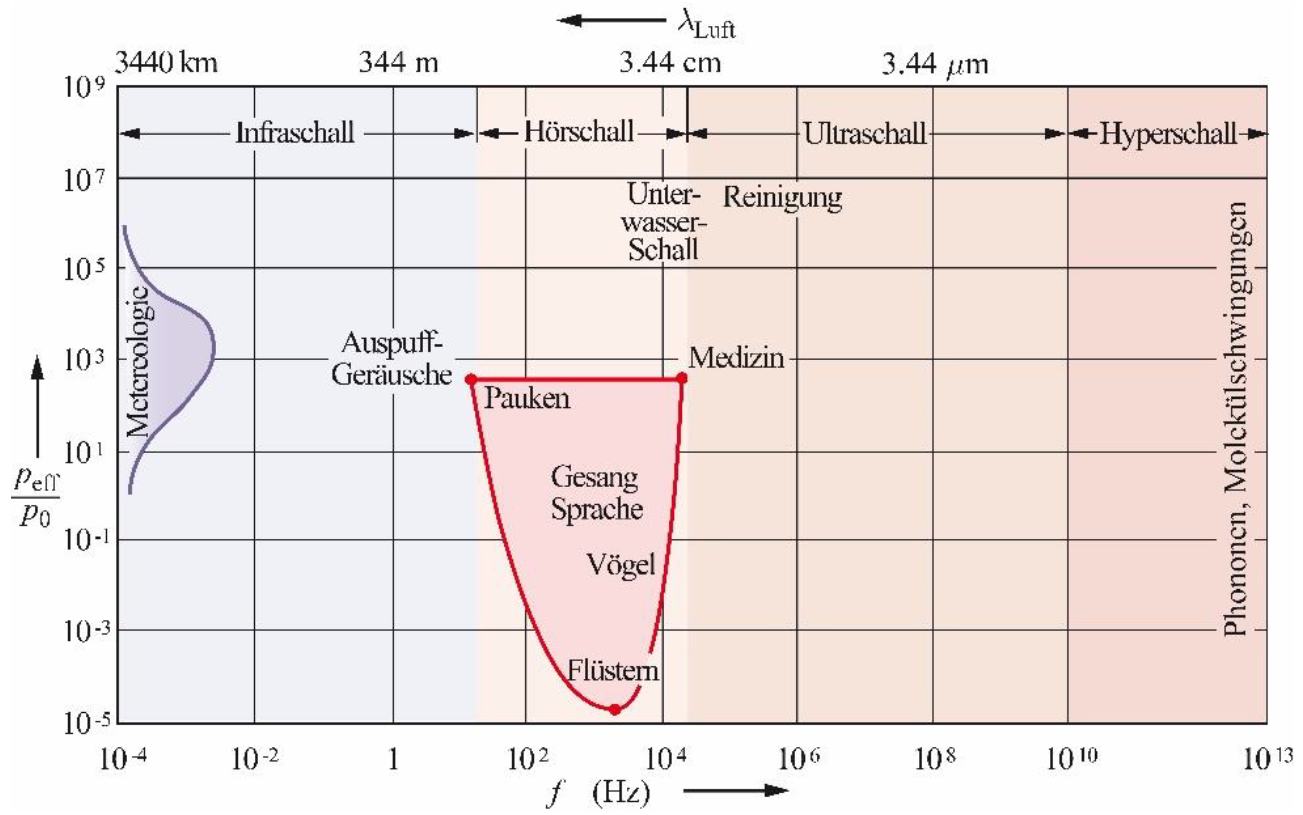
\includegraphics[width=0.9\linewidth]{Bilder/Wellen-Optik/schallquellen} \\

\subsection{PHON-Skala}
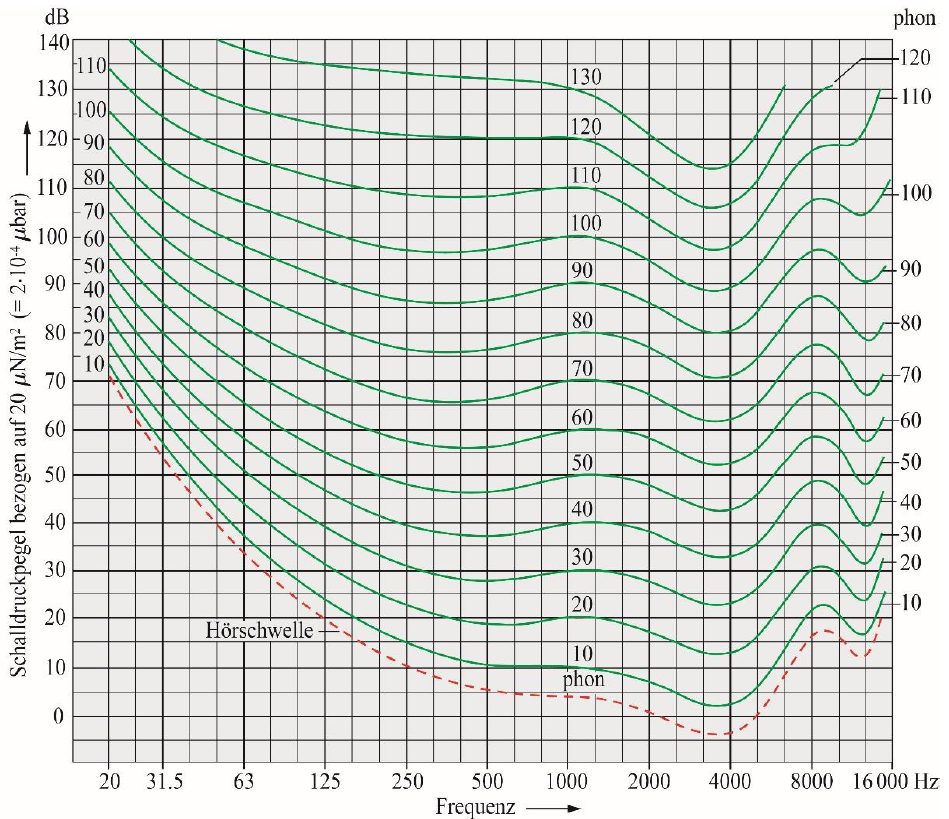
\includegraphics[width=0.95\linewidth]{Bilder/Wellen-Optik/phon_skala}



\subsection{Schalldämpfung / Schalldämmung}

\subsubsection{Schalldämpfung}

Schalldämpfung bedeutet eine \textbf{Abschwächung} der Schallwellen durch
\textbf{Absorption}. \\ Schallenergie wird in \textbf{'Wärme' umgewandelt}, d.h. durch die
Absorption von Energie werden das von den Schallwellen
durchdrungene Medium oder die das Schallfeld begrenzenden Körper
\textbf{erwärmt}. \\
\vspace{0.2cm}

\textbf{Verschiedene Arten von Absorption für Schalldämpfung Innen} \\

\begin{itemize}
	\itemsep0em
	\item Poröse Schicht (mit oder ohne perforierte Abdeckung) 
	\item Akustikplatte 
	\item Plattenresonator
	\item Helmholtz-Resonator
\end{itemize}

% \vfill\null
% \columnbreak

\subsubsection{Schalldämmung} 

Schalldämmung ist die \textbf{Behinderung der Schallausbreitung} durch
\textbf{reflektierende} Hindernisse. Mauern, Türen und Fenster bewirken eine
Schalldämmung für den von aussen in das Gebäude eindringenden
Schall. Auch die Ausbreitung von Schall innerhalb eines Gebäudes wird
durch die Schalldämmung von Zwischenwänden und Türen
abgeschwächt. Im Freien wird durch Schallschutzwände eine
Schalldämmung für die dahinterliegenden Gebäude erreicht.



\subsection{Schalldämmung / Schalldämm-Mass}

Bei der Schallübertragung muss zwischen \textbf{Luftschall} und \textbf{Körperschall}
unterschieden werden.

\subsubsection{Luftschalldämmung}

Es gibt Schallquellen, die ihre Schallenergie (fast)
ausschliesslich in die Luft abstrahlen.\\
Beispiele: menschliche Stimme, Geigen, Lautsprecher und Blasinstrumente

\subsubsection{Körperschalldämmung}

Andere Schallerzeuger übertragen die Schallschwingungen nicht nur auf die
Luft, sondern auch direkt auf feste Körper. Streichinstrumente, wie Cello oder
Bassgeige, und Klavier oder Flügel übertragen die Schallschwingungen auch
direkt auf den Fussboden. Wird ein Nagel in die Wand geschlagen, so wird ein
grosser Anteil des erzeugten Schalls als Körperschall übertragen. \\
Beispiele: Trittschall, Wasserleitungsgeräusche \\

% \vfill\null
% \columnbreak



\subsection{Schalldämm-Mass}

$$ \boxed{ \mathcal{R} = 10 \cdot \log\left( \frac{P_1}{P_2} \right)  } $$



\subsection{Anhall / Nachhall}

\subsubsection{Anhall}

Es dauert eine gewisse Zeit, bis sich eine \text{konstante Energiedichte} der Schallwellen \text{im Raum aufgebaut} hat. Dieser Vorgang wird Anhall genannt. Wegen der logarithmischen Empfindlichkeit des Ohrs \text{wird er praktisch nicht wahrgenommen}.

\subsubsection{Nachhall}

Die von den Begrenzungsflächen des Raumes mehrfach reflektierten Wellen bewirken andererseits, dass beim \text{plötzlichen Abschalten} einer Schallquelle der Schall nicht sofort verschwindet, sondern \text{allmählich abklingt}. Dieses Phänomen wird Nachhall genannt und ist im Gegensatz zum Anhall \text{deutlich wahrnehmbar}. \\
\vspace{0.2cm}

\textbf{Per Definition ist die Nachhallzeit jene Zeitspanne, in welcher der Schallpegel im Raum um 60 dB sinkt.}


\subsubsection{Nachhallzeit $T_N$}


$$ \boxed{ T_N = 0.16 \, \frac{\s}{\m} \frac{V}{\sum\limits_i \alpha_i A_i } } $$ \\

% \renewcommand{\arraystretch}{1.3}
\begin{tabular}{clc}
$T_N$ & Nachhallzeit & $[T_N] = \s$ \\
$V$ & Raumvolumen & $[V] = \m^3$ \\
$\alpha_i$ & Absorptionsgrad & $[\alpha_i] = 1$ \\
$A_i$ & Teilfläche der Raumbegrenzung & $[A_i] = \m^2$ \\ 
& mit Absorption $\alpha_i$ \\
\end{tabular}
% \renewcommand{\arraystretch}{1}

% \vfill\null
% \columnbreak